\chapter{Bavaria ancient DNA}
\label{chapterlabel4}

\section{Introduction}

Throughout the Pleistocene and Holocene, Germany has been the setting for many population movements and admixture events of modern humans; the Swabian Alps is home to one of the earliest symbolic art, dated to at least 32kya \cite{conard2009female} and musical instruments dated to 40kya \cite{conard2009new}, both assigned to the Aurignacian tradition. Later, the region was also home to one of the first Neolithic traditions in the \textit{Linearbandkeramik}, a key culture in the Neolithisation of Europe. 

Cherry-Tree cave (Kirschbaumhöhle in German) represents a perfect opportunity to study the transect of samples from the Neolithic to the present-day. The cave represents a relatively untouched layer of stratigraphy.

In the present-day, Germany represents a boundary point between East and West Europe; current population structure. Questions remain as to the origin of this East-West structure; is it recent structure, or does it persist to the Middle Ages or earlier? 

Here, I present novel data from 11 medium-to-hight coverage samples from two sites from Southern Germany and one site from one from Southern Austria. In particular, the samples from Kirschbaumhöhle span from the Late Neolithic to the Iron Age and represent an excellent opportunity to study a time transect. 

Previous studies into the genomic history of Bavaria have focused, for example, on the mixed ancestry of migrant females during the Early Middle Ages. 

I was interested in addressing the following questions:

\begin{enumerate}
\item \textbf{Second Neolithic immigration wave}. Do we observe genetic differences between the first and second wave of farmers that brought farming to the region technology from South-East Asia to Europe during the Early Neolithic?
\item \textbf{Cherry Tree Cave}. How can we make sense of the genetic ancestry changes from the Late Neolithic through to the Iron Age in Cherry Tree Cave? Do we see evidence of genetic continuity between the ages and are they characterised by admixture from outside sources?
\item \textbf{The Iron Age}. How do the samples from the Iron Age compare to the single sample from the Bronze Age,and both to central Europeans
\item \textbf{Iron Age - Middle Age} To what extent do the `proto-Celtic' samples of the Iron Age show similarity to the later early `Germanic' people of the middle ages.  
\item Is there a distinction between the Germanic and Slavic Middle Age samples? How do these populations compare to the preceding samples from the Bronze and Iron ages. 
\end{enumerate}

\section{Methods}

\subsection{Data generation}

11 whole-genomes of ancient individuals were generated by collaborators at the Johannes Gutenberg, University of Mainz, Germany. Their estimated radiocarbon dates range from 1060AD to 5200BC (Fig. \ref{fig:chapter4_intro_SamplesDates}). 6 of the samples were found in Cherry-Tree Cave in the Bavarian district of Forchheim (Fig. \ref{fig:chapter4_intro_SamplesMap}), 4 from futher South in the region of Dingolfing/Essenbach and one sample from southern Austria. The samples had a median coverage of 4.84x and ranged from 0.7x to 17.52x. Full details of coverage, location and dates are given in Table 4.1.

\begin{figure}[htp]
    \centering
    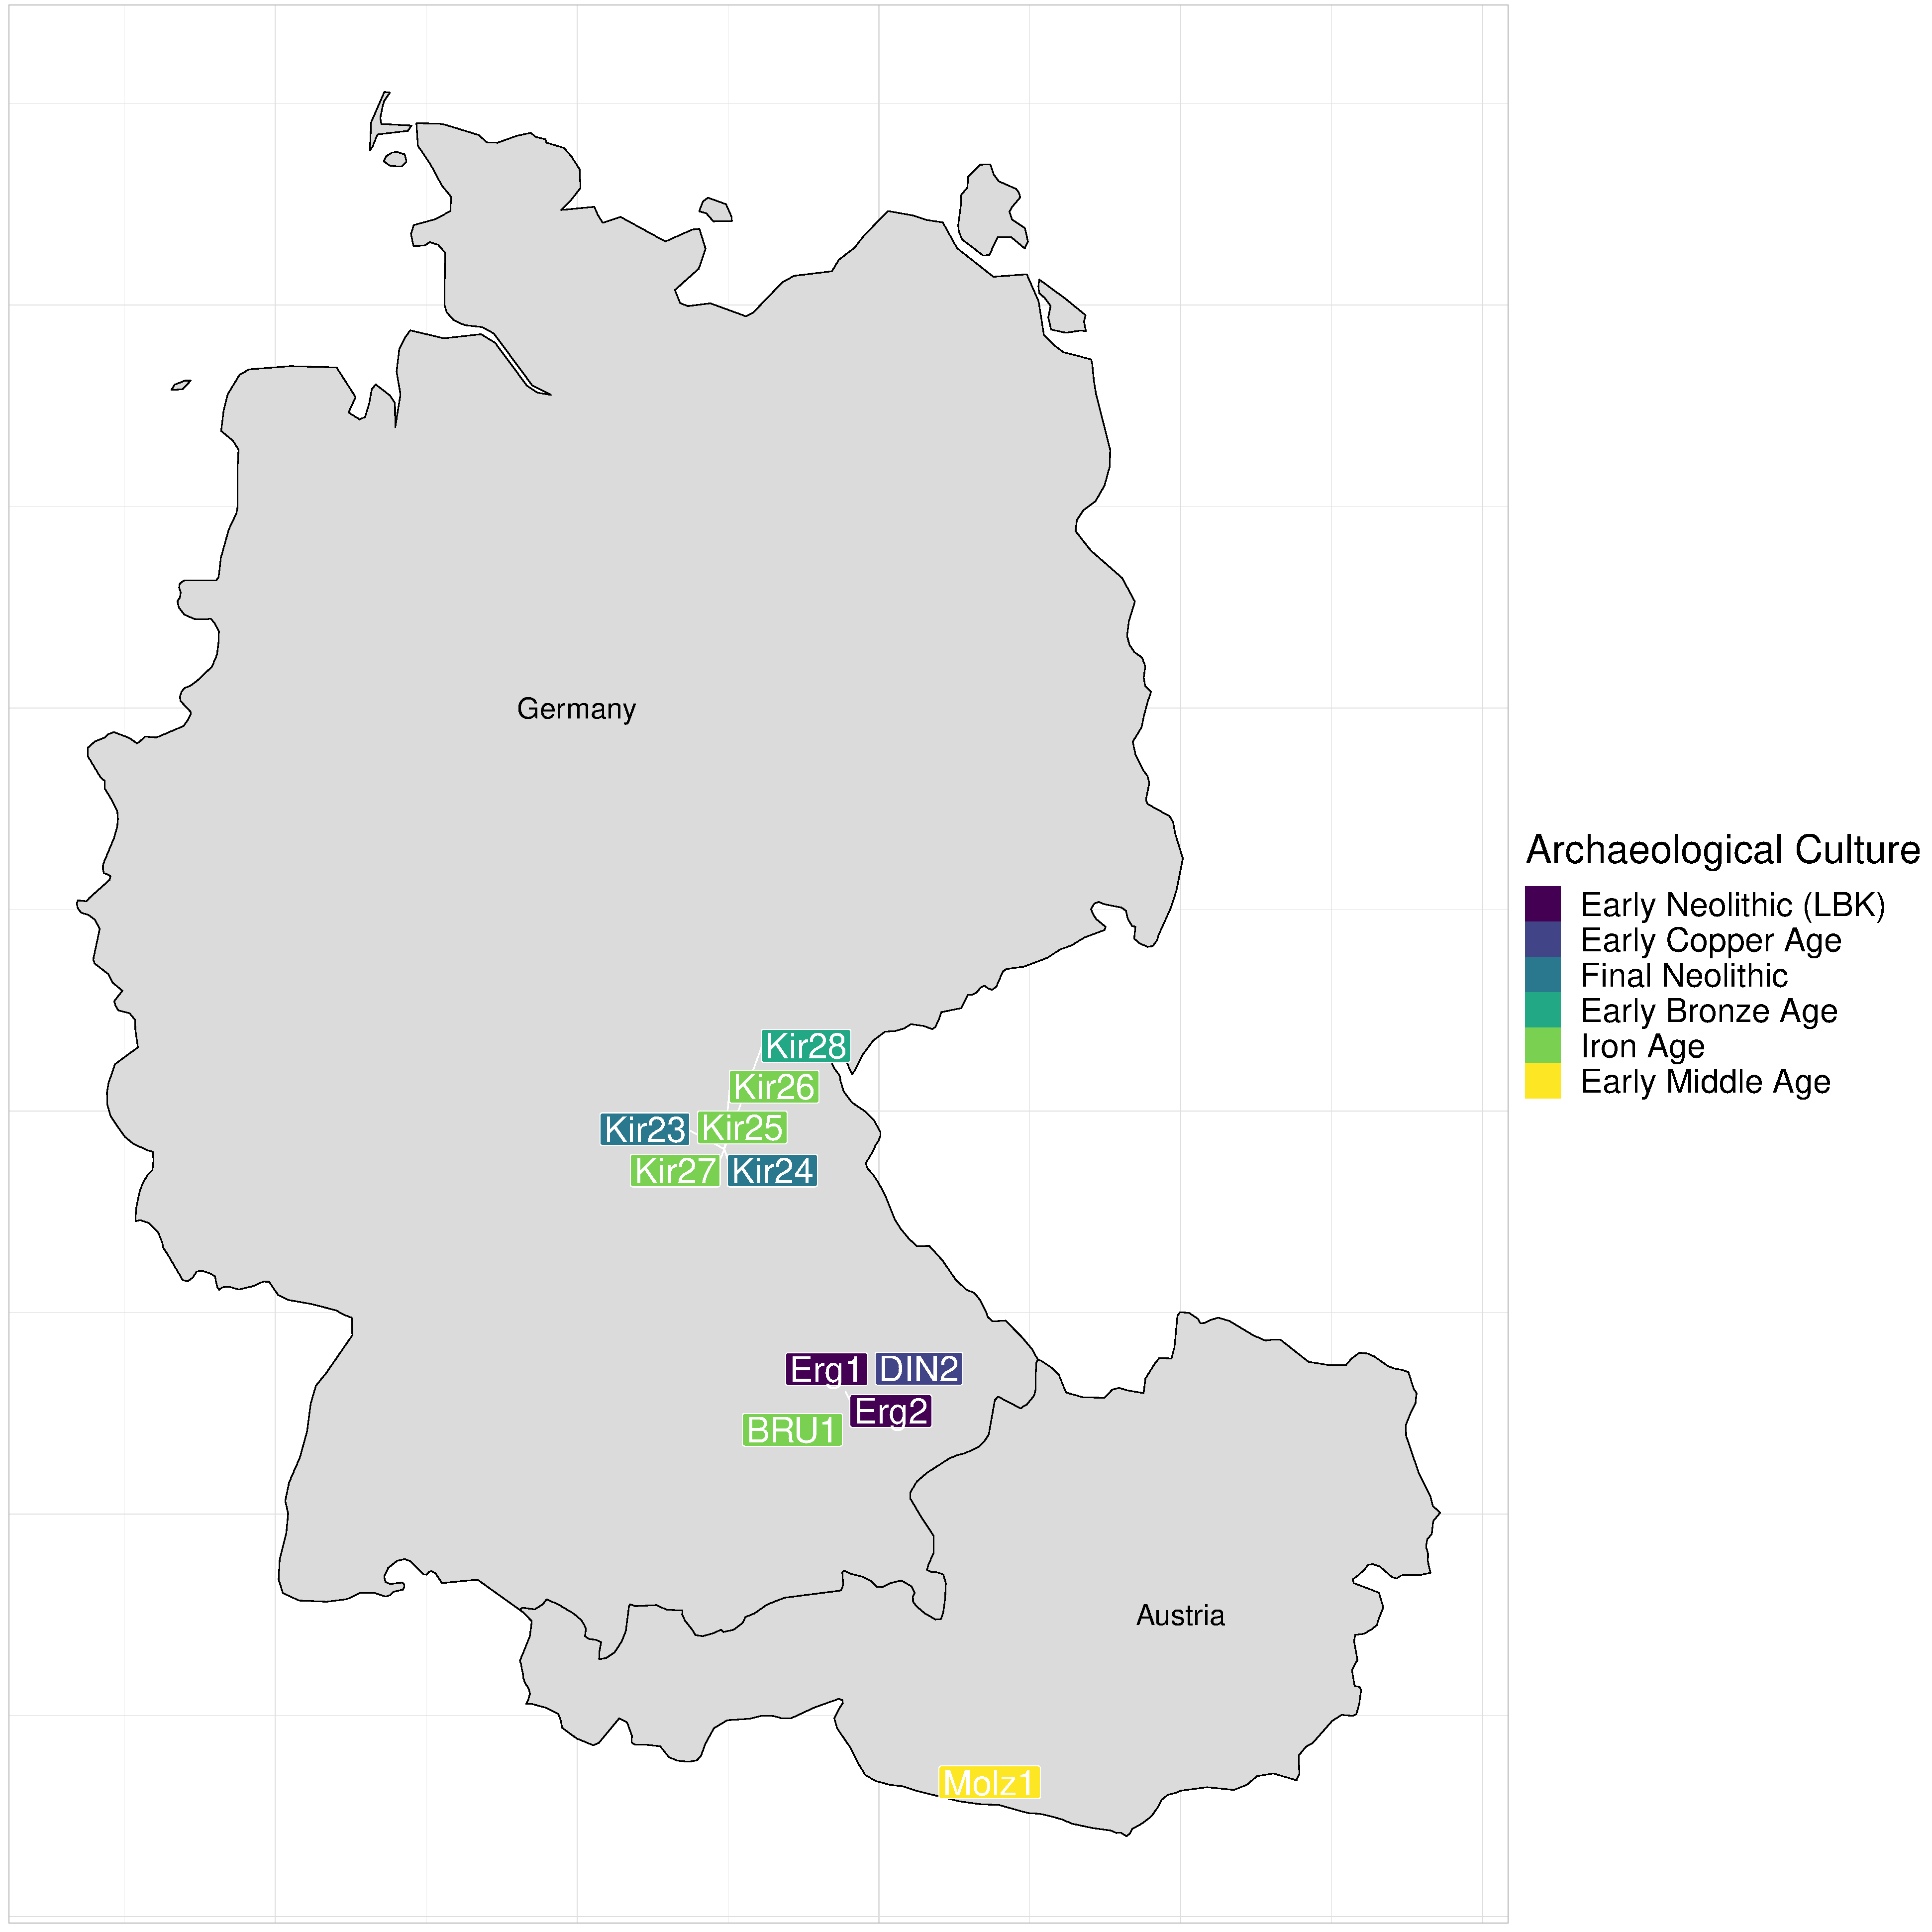
\includegraphics[width=1.0\textwidth]{../images/chapter4/sample_map.pdf}
    \caption{Map of newly sequenced ancient individuals, positioned according to where they were excavated. Colour on label corresponds to archaeological culture which they were found. }
    \label{fig:chapter4_intro_SamplesMap}
\end{figure}

\begin{figure}[htp]
    \centering
    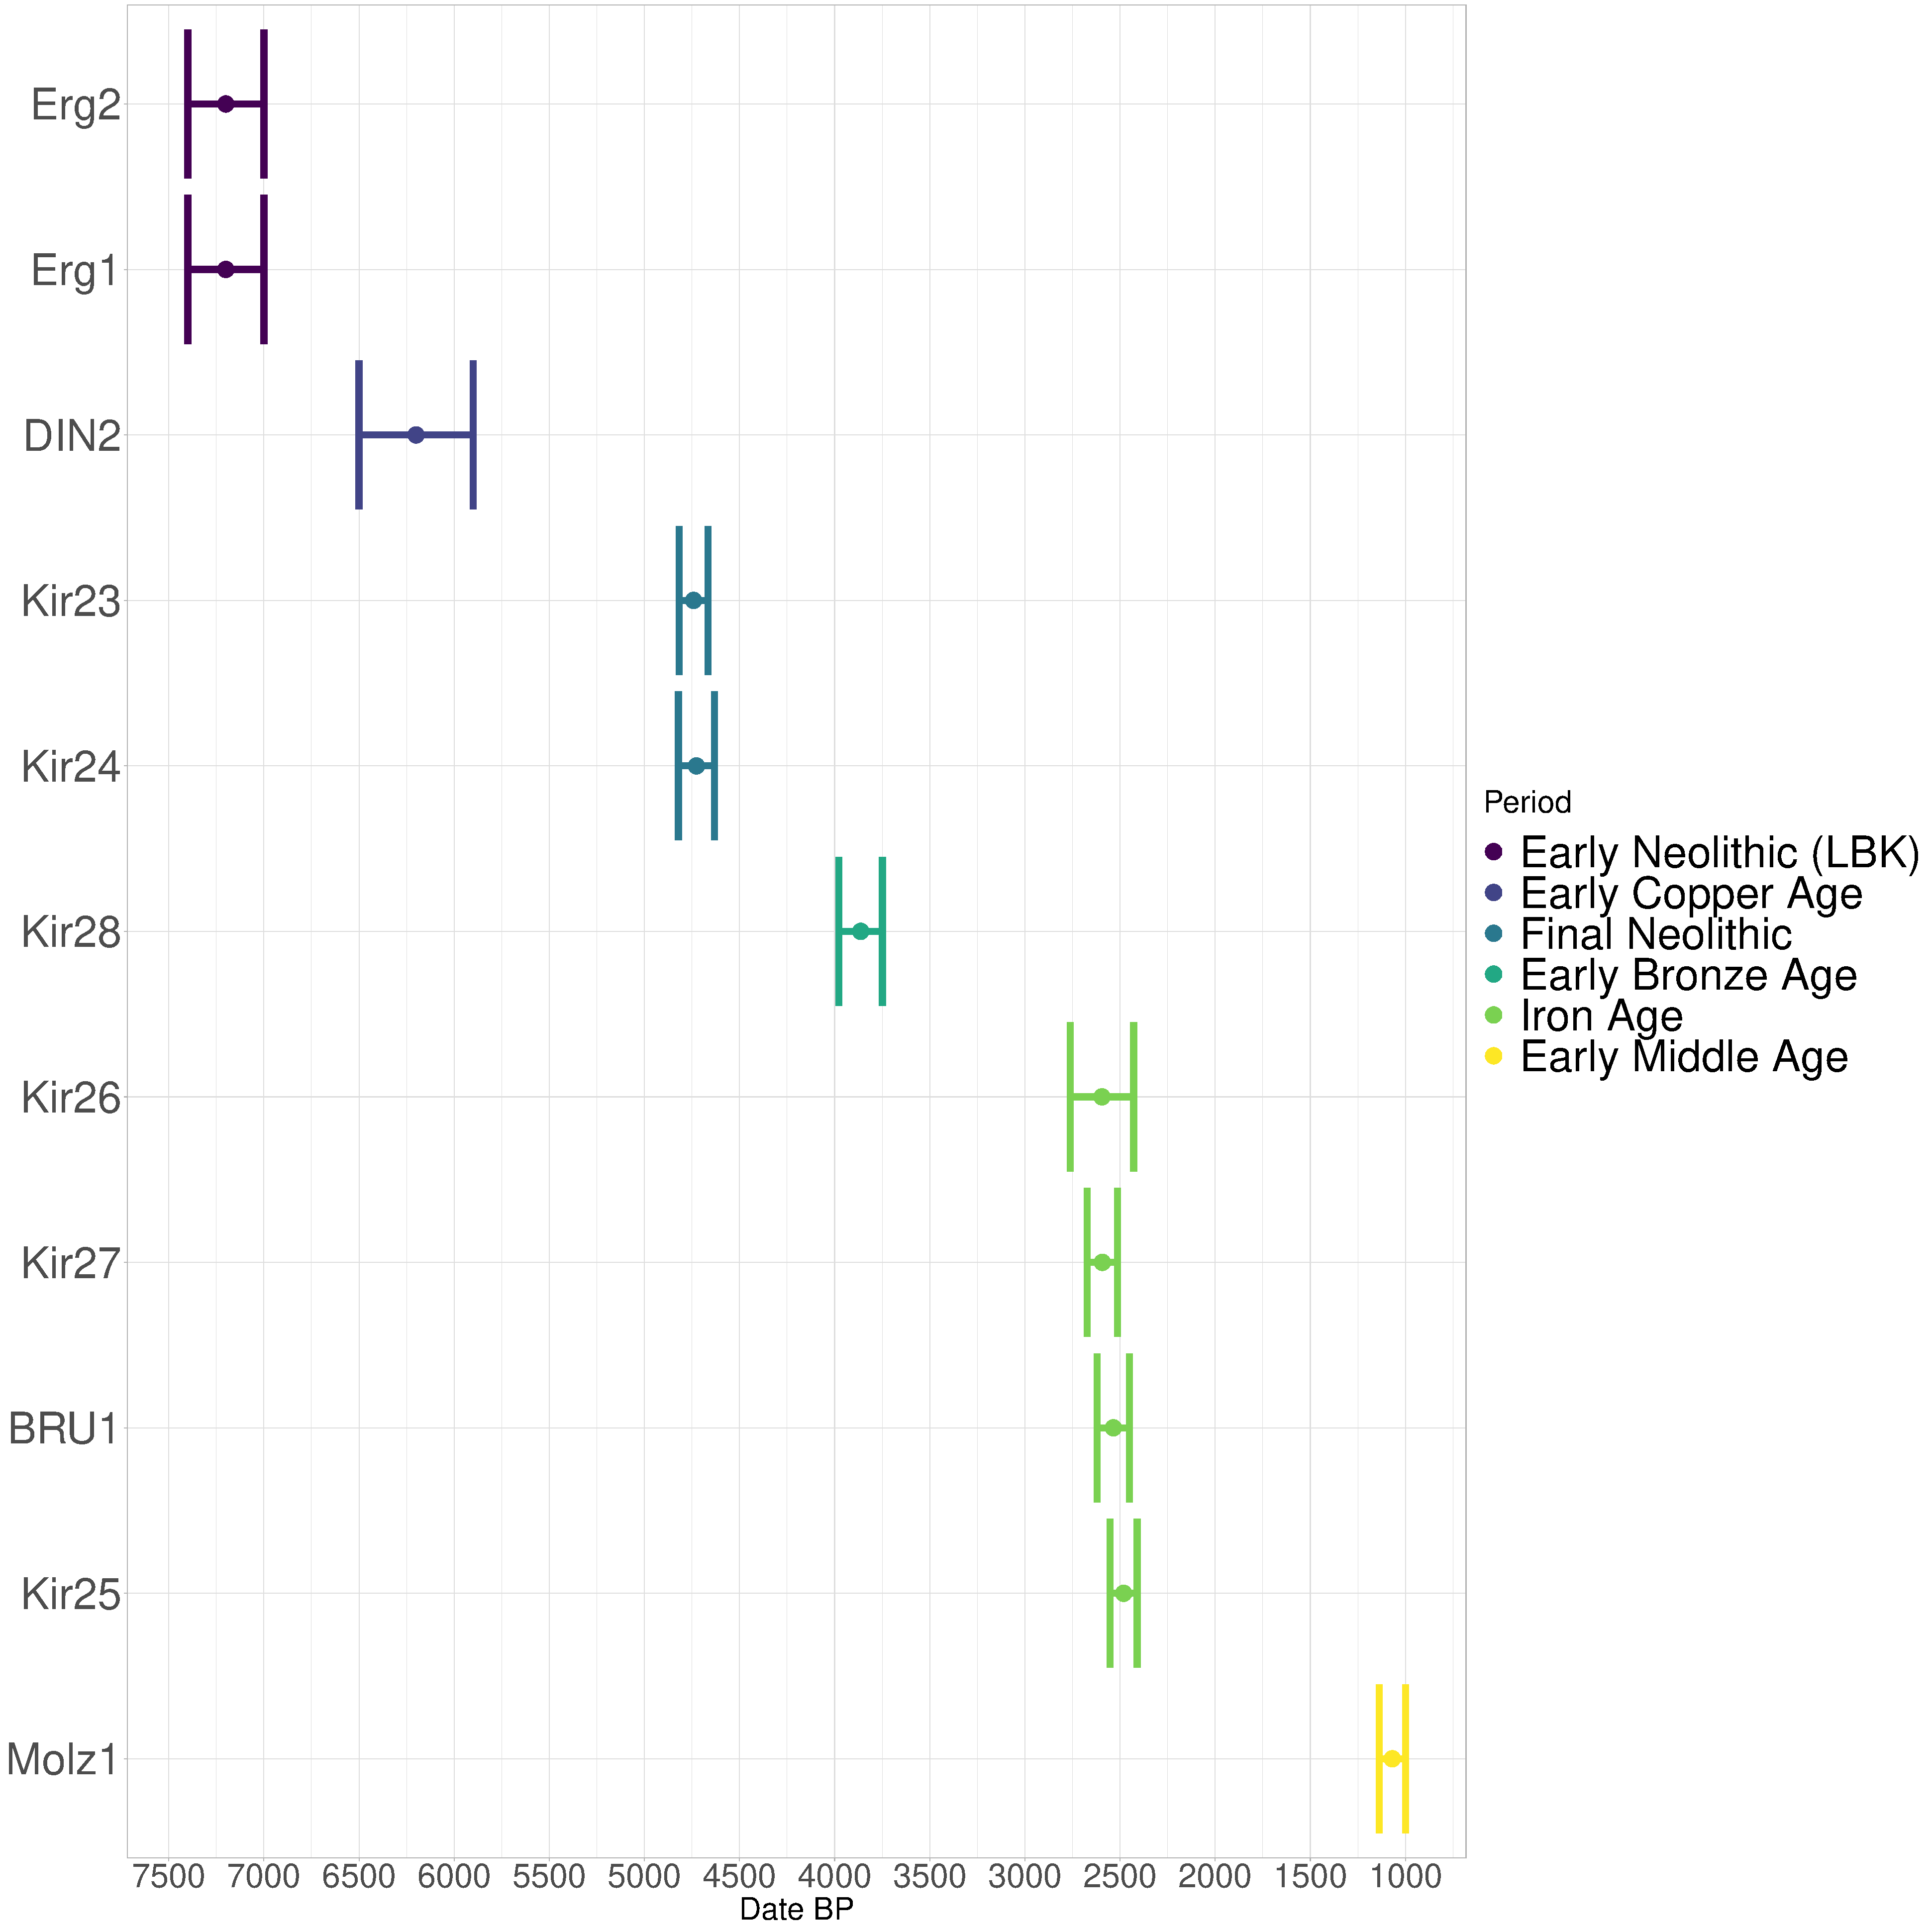
\includegraphics[width=1.0\textwidth]{../images/chapter4/Dates.pdf}
    \caption{Estimated radiocarbon dates for each newly sequenced ancient individual, grouped by archaeological period. }
    \label{fig:chapter4_intro_SamplesDates}
\end{figure}

\begin{table}
\small
\centering
\begin{tabular}{l|l|r|l|r}
\hline
Sample.ID & Location & Date & Period & Coverage \\
\hline
Erg1 & Ergoldsbach-Essenbach & 5200 & Early Neolithic (LBK) & 4.52\\
\hline
Erg2 & Ergoldsbach-Essenbach & 5200 & Early Neolithic (LBK) & 0.71\\
\hline
DIN2 & Dingolfing & 4200 & Early Copper Age & 1.71\\
\hline
Kir24 & Cherry Tree Cave & 2762 & Final Neolithic & 3.98\\
\hline
Kir23 & Cherry Tree Cave & 2741 & Final Neolithic & 17.52\\
\hline
Kir28 & Cherry Tree Cave & 1863 & Early Bronze Age & 17.30\\
\hline
Kir26 & Cherry Tree Cave & 595 & Iron Age & 4.84\\
\hline
Kir27 & Cherry Tree Cave & 593 & Iron Age & 16.60\\
\hline
BRU1 & Bruckberg & 535 & Iron Age & 11.54\\
\hline
Kir25 & Cherry Tree Cave & 481 & Iron Age & 4.55\\
\hline
Molz1 & Molzbichl & 1069 & Early Middle Age & 13.22\\
\hline
\end{tabular}
\caption{Table providing details for the newly sequenced Bavarian samples.}
\end{table}

\subsection{Stuff that Jens did (e.g. read aligning)}

Collaborators in University of Mainz performed DNA extraction, read alignment and variant calling. 

\subsection{Genotype imputation and phasing using GLIMPSE}
\label{sssec:imputationphasingGLIMPSE}

ChromoPainter analysis requires that all samples contain i) phased genotypes and ii) no missing genotypes. GLIMPSE \cite{rubinacci2021efficient} is a software which is designed to perform both phasing and imputation on low-coverage sequence data with the aid of a reference panel. GLIMPSE was chosen as it was the fastest phasing / imputation software available for low coverage sequence data avaliable at the time of writing \cite{rubinacci2021efficient}. The other possible option, Beagle4 \cite{Browning2007}, is too slow and memory inefficient to impute the large number combined number of individuals and SNPs present in this dataset. 

I merged the 11 newly sequenced individuals with the reference data-sets A.1 to A.17 resulting in a total of 942 individuals in \texttt{.bcf} format with genotype likelihood data at 77,213,942 genome-wide SNPs. Data was then split into separate \texttt{.bcf} files for each chromosome and indexed using bcftools \cite{li2009sequence}.

I followed the GLIMPSE \cite{rubinacci2021efficient} imputation and phasing pipeline (\url{https://odelaneau.github.io/GLIMPSE/tutorial_b38.html}) to generate genotype likelihoods and phased genotypes for each individual. For the reference panel, I used the 30x 1000 genomes dataset \cite{byrska2021high}, described in appendix A.5.  

\texttt{GLIMPSE chunk} was used to split the present-day reference dataset into chunks. Default settings of \texttt{--window-size 2000000} and \texttt{--buffer-size 200000} were used, generating a total of 936 regions genome wide. Splitting the genome into regions for imputation jointly maximises computational efficiency and accuracy \cite{rubinacci2021efficient}. For each region in turn, the target dataset, consisting of phred-scaled genotype likelihoods (PL), was imputed using \texttt{GLIMPSE phase} under default settings and the same reference panel. Here, `impute' means filling in sporadic missing genotypes that are missing in a single individual (or sometimes more), rather than the whole-scale imputation of non-genotyped positions. \texttt{GLIMPSE ligate} was then used to concatenate the 936 imputed regions into 22 distinct chromosomes. Finally, \texttt{GLIMPSE sample} was used to generate phased haplotypes from the output of \texttt{GLIMPSE ligate} using default settings. 50,342,061 bi-allelic autosomal SNPs remained after phasing and imputation. 

\subsection{Determination of uniparental haplogroups}

Haplogrep (\url{https://haplogrep.i-med.ac.at/}) was used to identify the mtDNA and y-chromosome haplogroups for each newly sequenced ancient samples \cite{weissensteiner2016haplogrep} from the raw \texttt{.fastq} files.

\subsection{Estimation sample-heterozygosity}

The phased haplotypes from the output of GLIMPSE were used to estimate per-sample heterozygosity using the \texttt{plink2 --het} command.

\subsection{IBD sharing}

I used hap-IBD \cite{zhou2020fast} to estimate IBD segments between all pairs of ancient individuals, using the phased output from GLIMPSE as input haplotypes, using the genetic maps supplied and leaving all parameters as default. I estimated IBD segments for each chromosome separately and summed their length segments between each pair of individuals across all chromosomes. 

\subsection{plink PCA}

To obtain a broad overview of the ancestry of the newly sequenced individuals in the context of 915 other ancient samples, I performed PCA on the pre-imputation genotypes using plink2. Performing a PCA in plink2 allows for the identification any data quality issues that are independent of phasing or ChromoPainter analysis. 

I retained the 500,000 markers with the lowest amount of missingness across all samples and LD-pruned the resulting SNPs using the settings \texttt{--maf 0.01} and \texttt{--indep-pairwise 50 5 0.2}. PCA was performed using default settings from plink2 and the first two principle components plotted.

\subsection{Chromopainter analysis}

To characterise of the ancestry of the newly sequenced ancient samples in the context of other ancient individuals.I first selected all ancient samples above 1.5x coverage (n=466) and performed an `all-v-all' painting where each haplotype was compared to all other haplotypes in turn. 1.5x was somewhat arbitrarily chosen as a conservative threshold to reduce coverage related bias whilst still retaining a suitable number of individuals. This is the painting that can be used to perform fineSTRUCTURE clustering and tree building on ancient samples. Hereafter referred to as `ancient' painting.

Principle Component Analysis was performed on the coancestry matrix of the `ancients' painting using the \texttt{prcomp\_irlba} function from the irlba R libary. Although there were 466 individuals in the `ancients' painting, not all of these were included in the chunklengths PCA. This was because many individuals in that set were not relevant to exploring the ancestry of the individuals at hand. For instance, when plotted, samples such as those from the Xiong Nu, a 3rd century BC culture from inner Mongolia, dominate the variation in a PCA to the point where identifying structure between the samples of interest becomes impossible. Therefore, a process of trial and error is used to decide which individuals to include in a PCA. This process is somewhat subjective, but occasionally subjective methods are required when facing heterogeneous ancient DNA datasets. 

I also performed an `all-v-all' painting of a selected group of present-day individuals and the newly sequenced ancient individuals. The populations retained are given in Table 4.2. Hereafter referred to as `present-day painting'.

\begin{table}
\small
\begin{tabular}{l|r}
\hline
Population & nsamples\\
\hline
HB:tsi & 196\\
\hline
HB:spanish & 68\\
\hline
HB:bulgarian & 62\\
\hline
HB:german & 60\\
\hline
HB:french & 56\\
\hline
HB:russian & 50\\
\hline
HB:greek & 40\\
\hline
HB:ukrainian & 40\\
\hline
HB:croatian & 38\\
\hline
HB:hungarian & 38\\
\hline
HB:norwegian & 36\\
\hline
HB:southitalian & 36\\
\hline
HB:polish & 34\\
\hline
HB:romanian & 32\\
\hline
HB:mordovian & 30\\
\hline
HB:cypriot & 24\\
\hline
HB:northitalian & 24\\
\hline
HB:lithuanian & 20\\
\hline
HB:siciliane & 20\\
\hline
HB:westsicilian & 20\\
\hline
HB:belorussian & 18\\
\hline
HB:tuscan & 16\\
\hline
HB:irish & 14\\
\hline
HB:scottish & 12\\
\hline
HB:germanyaustria & 8\\
\hline
HB:welsh & 8\\
\hline
\end{tabular}
\caption{Name of population and number of samples used in the present-day ChromoPainter analysis}
\end{table}

I selected the MS POBI HellBus dataset of present-day individuals, described in Appendix A.21, to co-analyse the newly sequenced ancient individuals with, as it contains a large number of European individuals which are relevant to studying the history of Germany. Appendix A.21 describes the phasing and pre-processing performed on this dataset. Once phased, I converted it to ChromoPainter format using a custom script (\url{https://github.com/sahwa/vcf_to_chromopainter}). I then merged the ancient individuals, described in sections \ref{sssec:imputationphasingGLIMPSE}, with the MS POBI HellBus dataset. I retained all bi-allelic SNPs common to both datasets, resulting in 414,155 SNPs.

Both the `present-day' and `ancient' paintings were merged separately using chromocombine-0.0.4 (\url{https://people.maths.bris.ac.uk/~madjl/finestructure-old/chromocombine.html}). 

The fineSTRUCTURE (v0.0.5)\cite{Lawson2012} clustering and tree building algorithm was applied to the chunkcounts ChromoPainter output for the `ancient' painting. This algorithm assigns individuals to genetically homogeneous clusters, estimates the `true' number of clusters and builds a dendrogram of genetic similarity. This is particularly useful when combining many samples from different studies, as is the case with the `ancients' painting; the population label identifiers used by different studies may not be consistent with one another. Therefore, we can use fineSTRUCTURE groupings as population labels rather than external group labels. fineSTRUCTURE was first run in MCMC mode using 1,000,000 burn-in MCMC iterations and 2,000,000 main MCMC iterations. It was then run in tree-building mode (\texttt{-m T}) using 100,000 burn-in and 100,000 main iterations. 

Tree figures, co-ancestry matrix figures and principle component plots were generated using the fineSTRUCTURE R library \url{(https://people.maths.bris.ac.uk/~madjl/finestructure/FinestructureRcode.zip)}.

\subsection{SOURCEFIND}

The coancestry matrices outputted by ChromoPainter give informative but noisy estimates of the how much recent ancestry a given individual most closely shares with another individual. This noise is due to in part to incomplete lineage sorting. SOURCEFIND \cite{Chacon-Duque2018} is a method of de-noising the ancestry estimates outputted by ChromoPainter. In SOURCEFIND nomenclature, `surrogates' are populations for which we wish to estimate proportions of ancestry of in our target population. For instance, in the most simple case, we may wish to estimate the proportion of `African' and `European' ancestry within an admixed target individual. There, we would use 2 surrogates, perhaps a population from Yoruba and a population from France. The surrogates need not be the `true' mixing sources. It is important to to note that SOURCEFIND does not directly infer admixture events, in that it does not model the break down of admixture LD as does ALDER or GLOBETROTTER. 

I performed 3 different SOURCEFIND analyses, each with a different set of surrogates.

Previous research suggests that almost all ancient Europeans (discounting particular paleolithic Hunter-Gather populations \cite{Fu2016}) can be well modeled as differing amounts of Western Hunter Gatherers (WHG), Early Neolithic farmers from present-day Anatolia and Bronze Age pastoralists from the Eurasian Steppe (best represented by individuals from the Yamnaya culture \cite{Lazaridis2014}). Therefore, a simple approach to identifying the broad-scale ancestry of ancient individuals is to model them as a mixture of the three aforementioned populations. I performed SOURCEFIND analysis, using these 3 populations as surrogates.

I also estimated finer-scale ancestry proportions by modeling each newly sequenced ancient sample as a mixture of all ancient populations which are older than the target. I chose to use only older surrogate populations as modeling an individual in terms of more recent populations can lead to results which are more difficult to directly interpret. I retained surrogate populations where the average age of samples within the population was older or within 100 years of the target individual. Accordingly, different newly sequenced ancient samples were analysed using different number of surrogate populations. 

Finally, I wanted to estimate proportions of ancestry from present-day surrogates in ancient samples. For this analysis, I used the `modern' painting and used all modern populations from the `HellBus' dataset as surrogates, shown in Table 4.2.

For all of the three above analyses, I performed 3 independent SOURCEFIND runs. SOURCEFIND explores the parameter space of ancestry proportions using MCMC sampling. For each target, all 3 MCMC runs were then combined to form an MCMC list using the \texttt{coda} R library \cite{oro22547}. I used the \texttt{mcmc} function to jointly estimate ancestry proportions and empirical credible intervals for each target population. 

\subsection{MOSAIC admixture analysis}

I inferred admixture events, dates and proportions using MOSAIC, a haplotype-based method \cite{MOSAIC_2019}. MOSAIC was used because, unlike GLOBETROTTER \cite{Hellenthal2014}, the `painting' step and admixture inference step are combined into one, resulting in a simpler pipeline and more flexible assignment of different surrogates (i.e. the set of surrogates can be changed without repainting the samples). MOSAIC also estimates $f_{st}$ between the set of surrogates and the estimated `true' mixing source, which is useful when a close proxy for the `true' mixing source is not available. 

I performed 2 different kinds of admixture analysis. Firstly, I performed an `ancient surrogates' analysis where the all ancient samples above 1.5x coverage were used as surrogates. I used the fineSTRUCTURE groupings to assign the samples into surrogate population.

I then performed a `present-day surrogates' analysis where a selected set of present-day populations were used to analyse both present-day Slavic populations and ancient Slavic populations. From prior experience, using these samples provided less-noisy results (due to larger population sample sizes and more homogenous populations), at the cost of reduced interpretability. By this, I mean that forming, for example, a 4,000 year-old Bronze Age sample as a mixture of present Europeans may be difficult to interpret; what does it mean if it is 70\% French and 30\% Tuscan? As the samples become more recent (i.e. into the Middle Ages), forming them as a mixture of moderns becomes more appropriate, since there has been relatively fewer large scale population movements separating the ancient and modern samples.

Phased \texttt{.vcf} files, the output from GLIMPSE, were converted to \texttt{.hap/.sample} files using \texttt{bcftools convert --hapsample}. The resulting \texttt{.hap/.sample} files were then converted to MOSAIC input using the provided script (\url{https://maths.ucd.ie/~mst/MOSAIC/convert_from_haps.R}). MOSAIC was run using default settings and the following sets of populations as targets and the following sets as surrogates. I formed each target as a mixture of either 2 or 3 ancestral sources. Upper and lower quantiles for admixture dates were estimated using a bootstrap procedure when more than one sample was present. Otherwise, when there is a single target sample, it is not possible to obtain confidence intervals.

\subsection{F-statistics}

Many of the relevant samples in the literature were of either very low coverage ($<0.1$) or genotyped on a capture array. Firstly, my in chapter 2 has shown that samples less than 0.5x cannot reliably be analysed using ChromoPainter. F-statistics (such as the $f_{3}$ admixture test or the $f_{4}$ branch test) are mostly robust to coverage related effects \cite{AssessingqpAdm}. Therefore, using these methods allows for the co-analysis of a much larger number of samples. In particular, there were many low-coverage samples from LBK cultures from Rivollat et al (2020) which would not have been suitable for use with ChromoPainter \cite{rivollat2020france}. The dataset used to calculate F-statistics contained 942 ancient samples from 143 populations, described in appendices A1 to A18, from the literature and 2280 present-day individuals from 144 populations from the HellBus dataset. 

I used Admixtools \cite{Patterson2012}, implemented in admixtools2 R library \url{(https://uqrmaie1.github.io/admixtools)} to calculate several different f-statistics. 

I converted imputed genotypes in \texttt{.vcf} format to \texttt{.ped}/\texttt{.map} format using plink. It has been shown that using imputed markers reduced reference bias relative to using pseudo-haploid markers \cite{Martiniano2017}. Convertf (\url{https://github.com/argriffing/eigensoft/tree/master/CONVERTF}) from the Admixtools library was then used to convert \texttt{.ped/.map} files into Eigenstrat format suitable for use with Admixtools. 

I used the $f_{4}$ branch test to test whether 2 populations form a clade to the exclusion of 2 other populations. For example, the $f_{4}(french,german;yoruba,mbuti)$ would give a $Z$ score not significantly different to zero, given we would expect $french$ and $german$ to form a clade to the exclusion of $yoruba$ and $mbuti$. Exchanging $french$ with $yoruba$ would yield $|Z| > 3$.

$f_{3}$ in the form of $f_{3}(A,B;C)$ was used to either i) estimate the branch length between $A$ and $B$ after their divergence from $C$, or ii) to test whether $C$ has been formed from an admixture event between $A$ and $B$, based on if $C$ has allele-frequencies which are intermediate between $A$ and $B$.

qpAdm was used to infer ancestry proportions. I followed the steps (as closely as was possible given the samples avaliable to me) taken in Olalde et al (2018) with respect to outgroup selection, choosing the following populations/samples: \textit{Mota}, \textit{Kostenki14}, \textit{papuan}, \textit{han}, \textit{hannchina}, \textit{mbutipygmy}, \textit{sannamibia}, \textit{yakut}. These outgroups were suitable for use in investigating ancient Eurasians, since they are asymmetrically related to many ancient populations, but do not show evidence of recent gene flow with them. 

\section{Results}

\subsection{Broad overview of genetic ancestry}

To obtain a broad overview of the genetic ancestry of the newly sequenced samples in the context of a large number of previously published ancient samples, I performed a principle component analysis on the genotype matrix of selected ancient samples using plink2 (Fig. \ref{fig:plink_PCA}). 

As expected, the samples from the Early Neolithic (approx 5200BC) and Copper Age (approx 4200BC) cluster with other samples from the European Neolithic. Previous studies have explained the pattern observed when Neolithic samples are plotted on a PCA \cite{Lipson2017b}; the earliest Neolithic samples, from Anatolia and Greece, who are thought to be the source population from which all subsequent Neolithic farmers derive \cite{Hofmanova2016, Haak2010, haak2005ancient, bramanti2009genetic, Lazaridis2014}, are usually positioned at the end of the cluster which is farthest away from the Bronze Age samples. This likely reflects the fact they are unadmixed and more drifted with respect to the later Neolithic samples. As the Neolithic progressed, farmers from the near-east mixed with local hunter-gatherer groups in central Europe \cite{Lipson2017b} and acquired local hunter-gatherer ancestry. Accordingly, these samples are shifted away from the earlier Neolithic samples, `north', towards the Bronze Age samples. I did not include hunter-gatherer samples in order to maximise the relevant space-efficiency of the PCA, but the later Neolithic samples would be shifted towards hunter-gatherer populations if present (see supplementary figure D.1). With this in mind, the position of Erg1, shifted north away from the contemporaneous sample Erg2, is suggestive of hunter-gatherer admixture. 

The 2 samples from the Late Neolithic display substantial differences; one sample, Kir24, is  positioned at the extreme top-left of the PCA, close to the Yamnaya type-specimen, indicating it shares very recent ancestry with the first Yamnaya individuals who carried `Steppe-related' ancestry from central Asia to Europe. On the other hand, Kir23 clusters with samples from Neolithic Europe. Kir28, the single Bronze Age sample clusters primarily with other European Bronze Age samples, whereas the 4 samples from the Iron Age are shifted substantially towards the Neolithic cluster, consistent with the placement of other samples from the European Iron Age. Finally, the 3 samples from the Medieval period, Alh1, Alh10 and Molz1, cluster with the Bronze Age. 

\begin{figure}[htp]
    \centering
    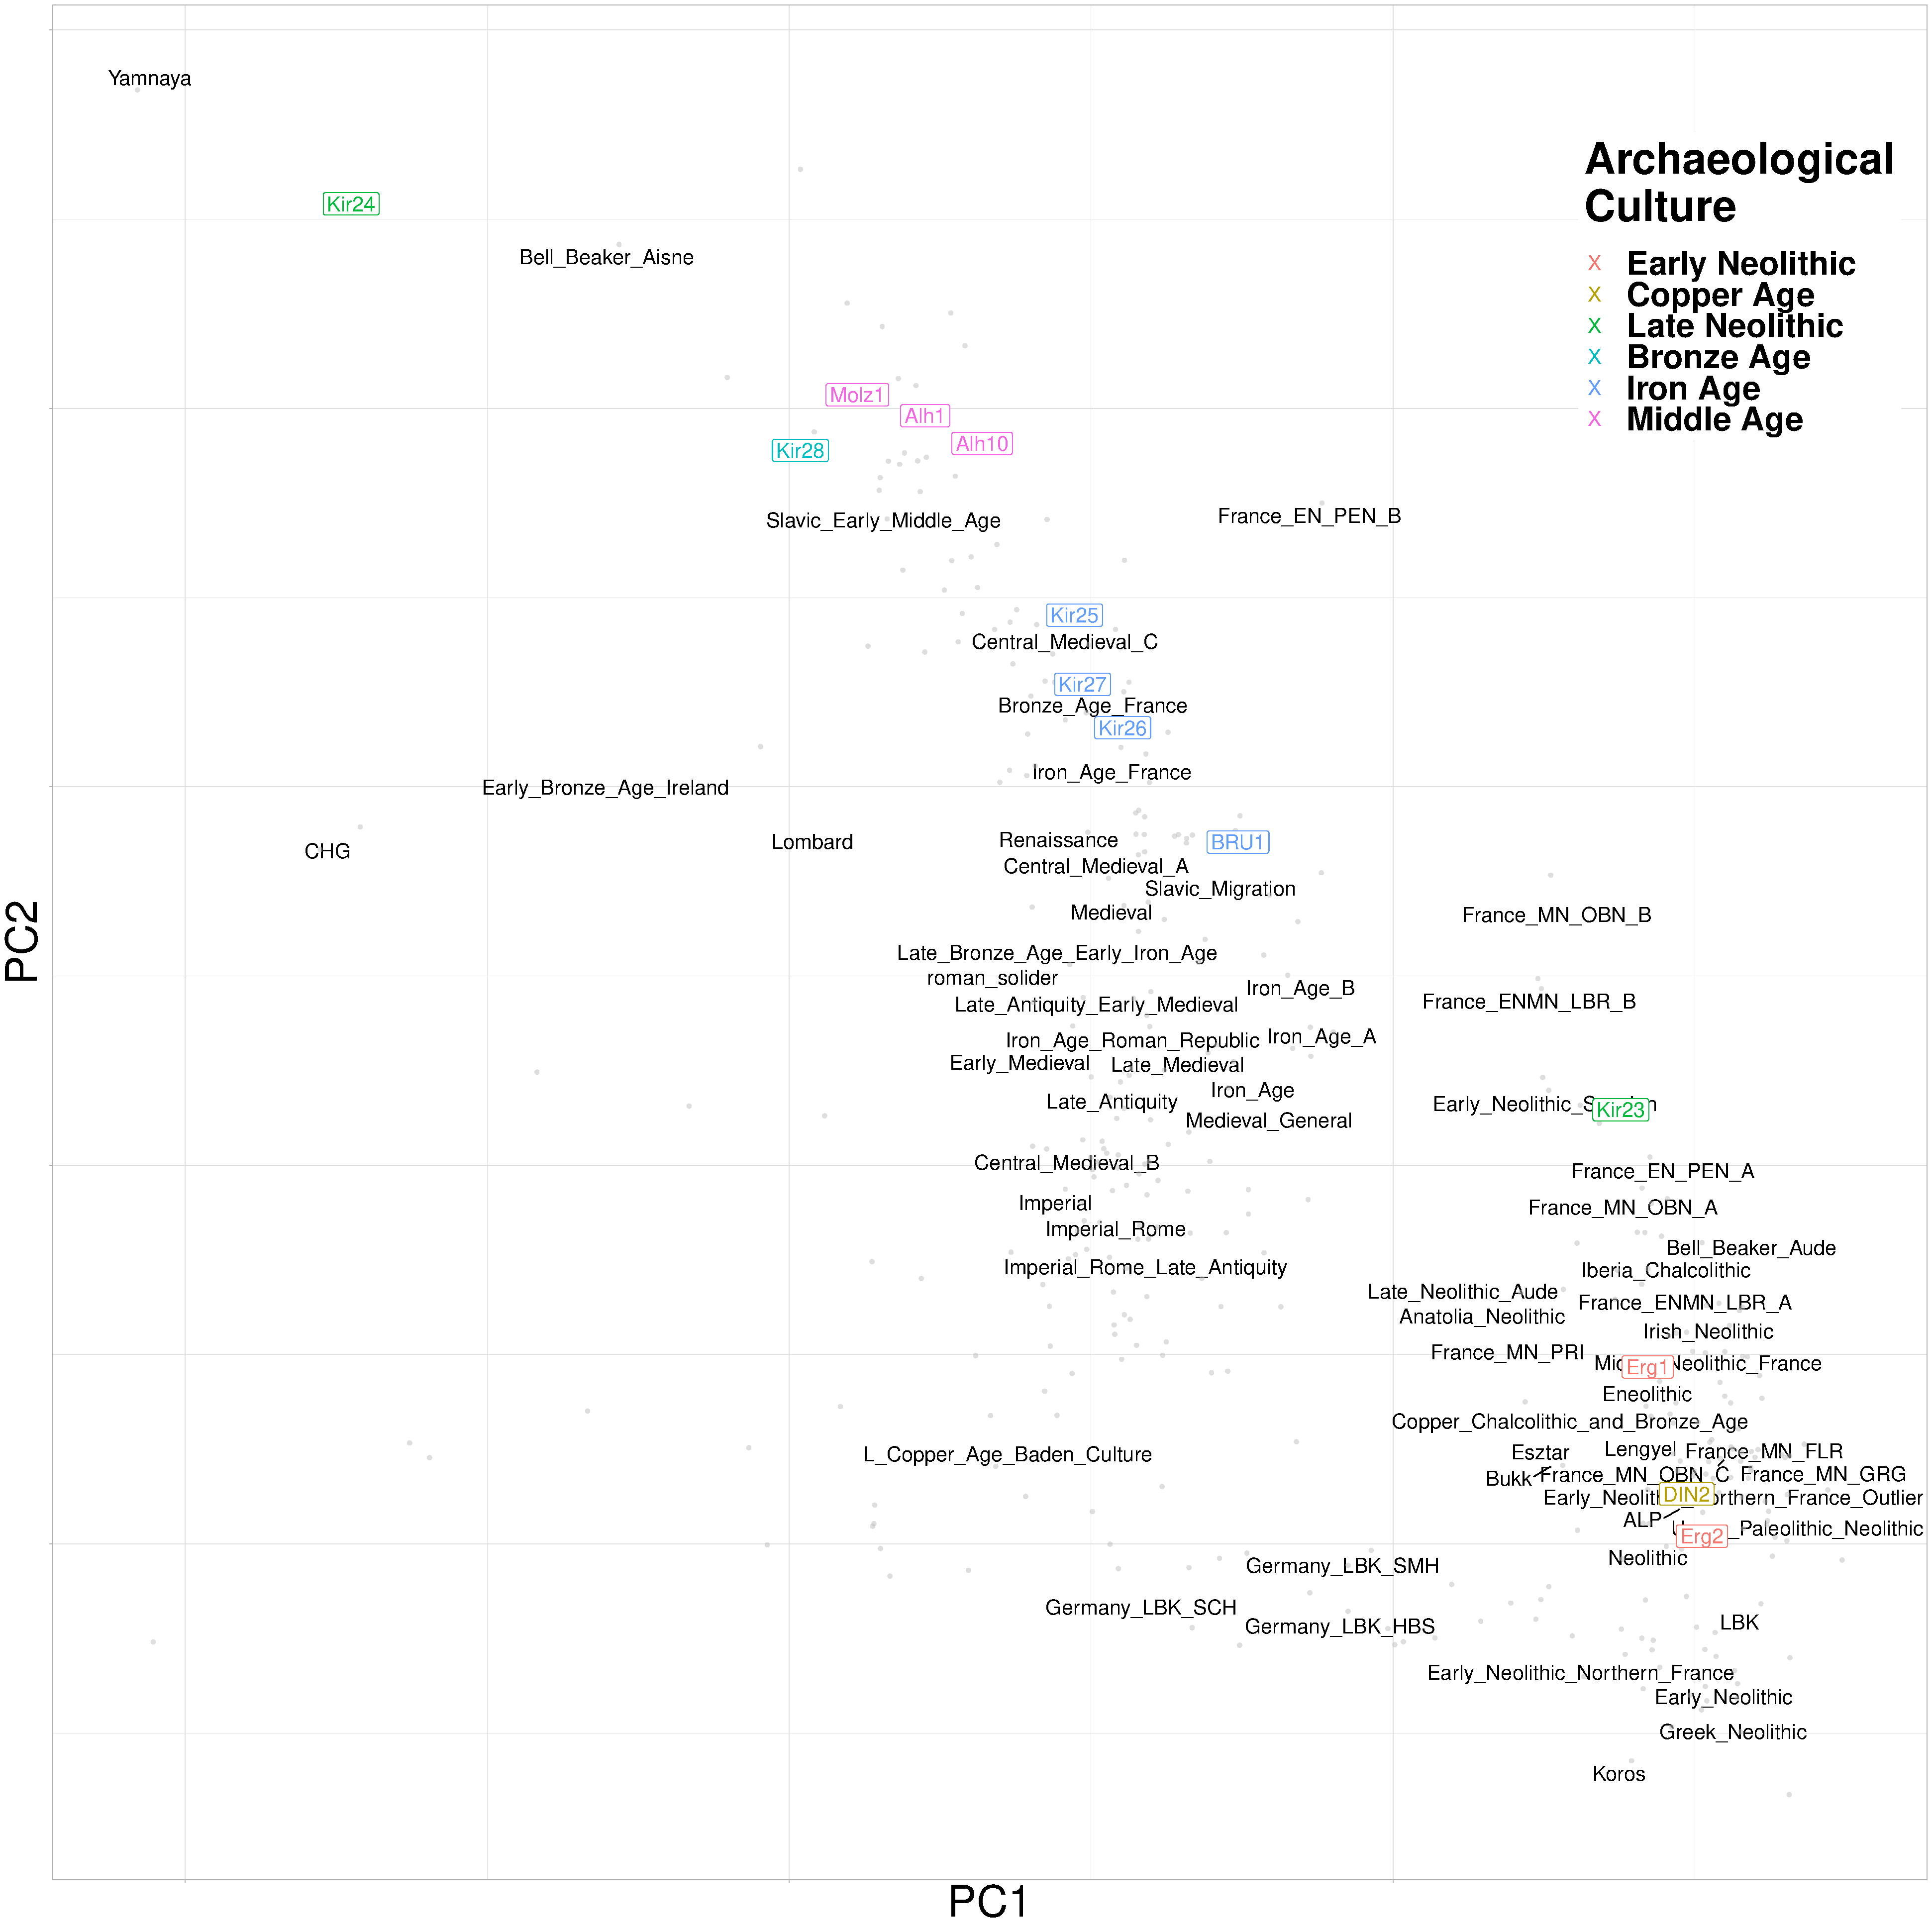
\includegraphics[width=1.0\textwidth]{../images/chapter4/plink_PCA.pdf}
    \caption{Principle component analysis of genotype matrix using plink2. Grey points indicate principle component coordiantes for each sample. Black text indicated mean principle component coordinates for all individuals within that group. Coloured labels represent newly sequenced ancient samples.}
    \label{fig:plink_PCA}
\end{figure}

\subsection{Early Neolithic}

\begin{figure}[htp]
    \centering
    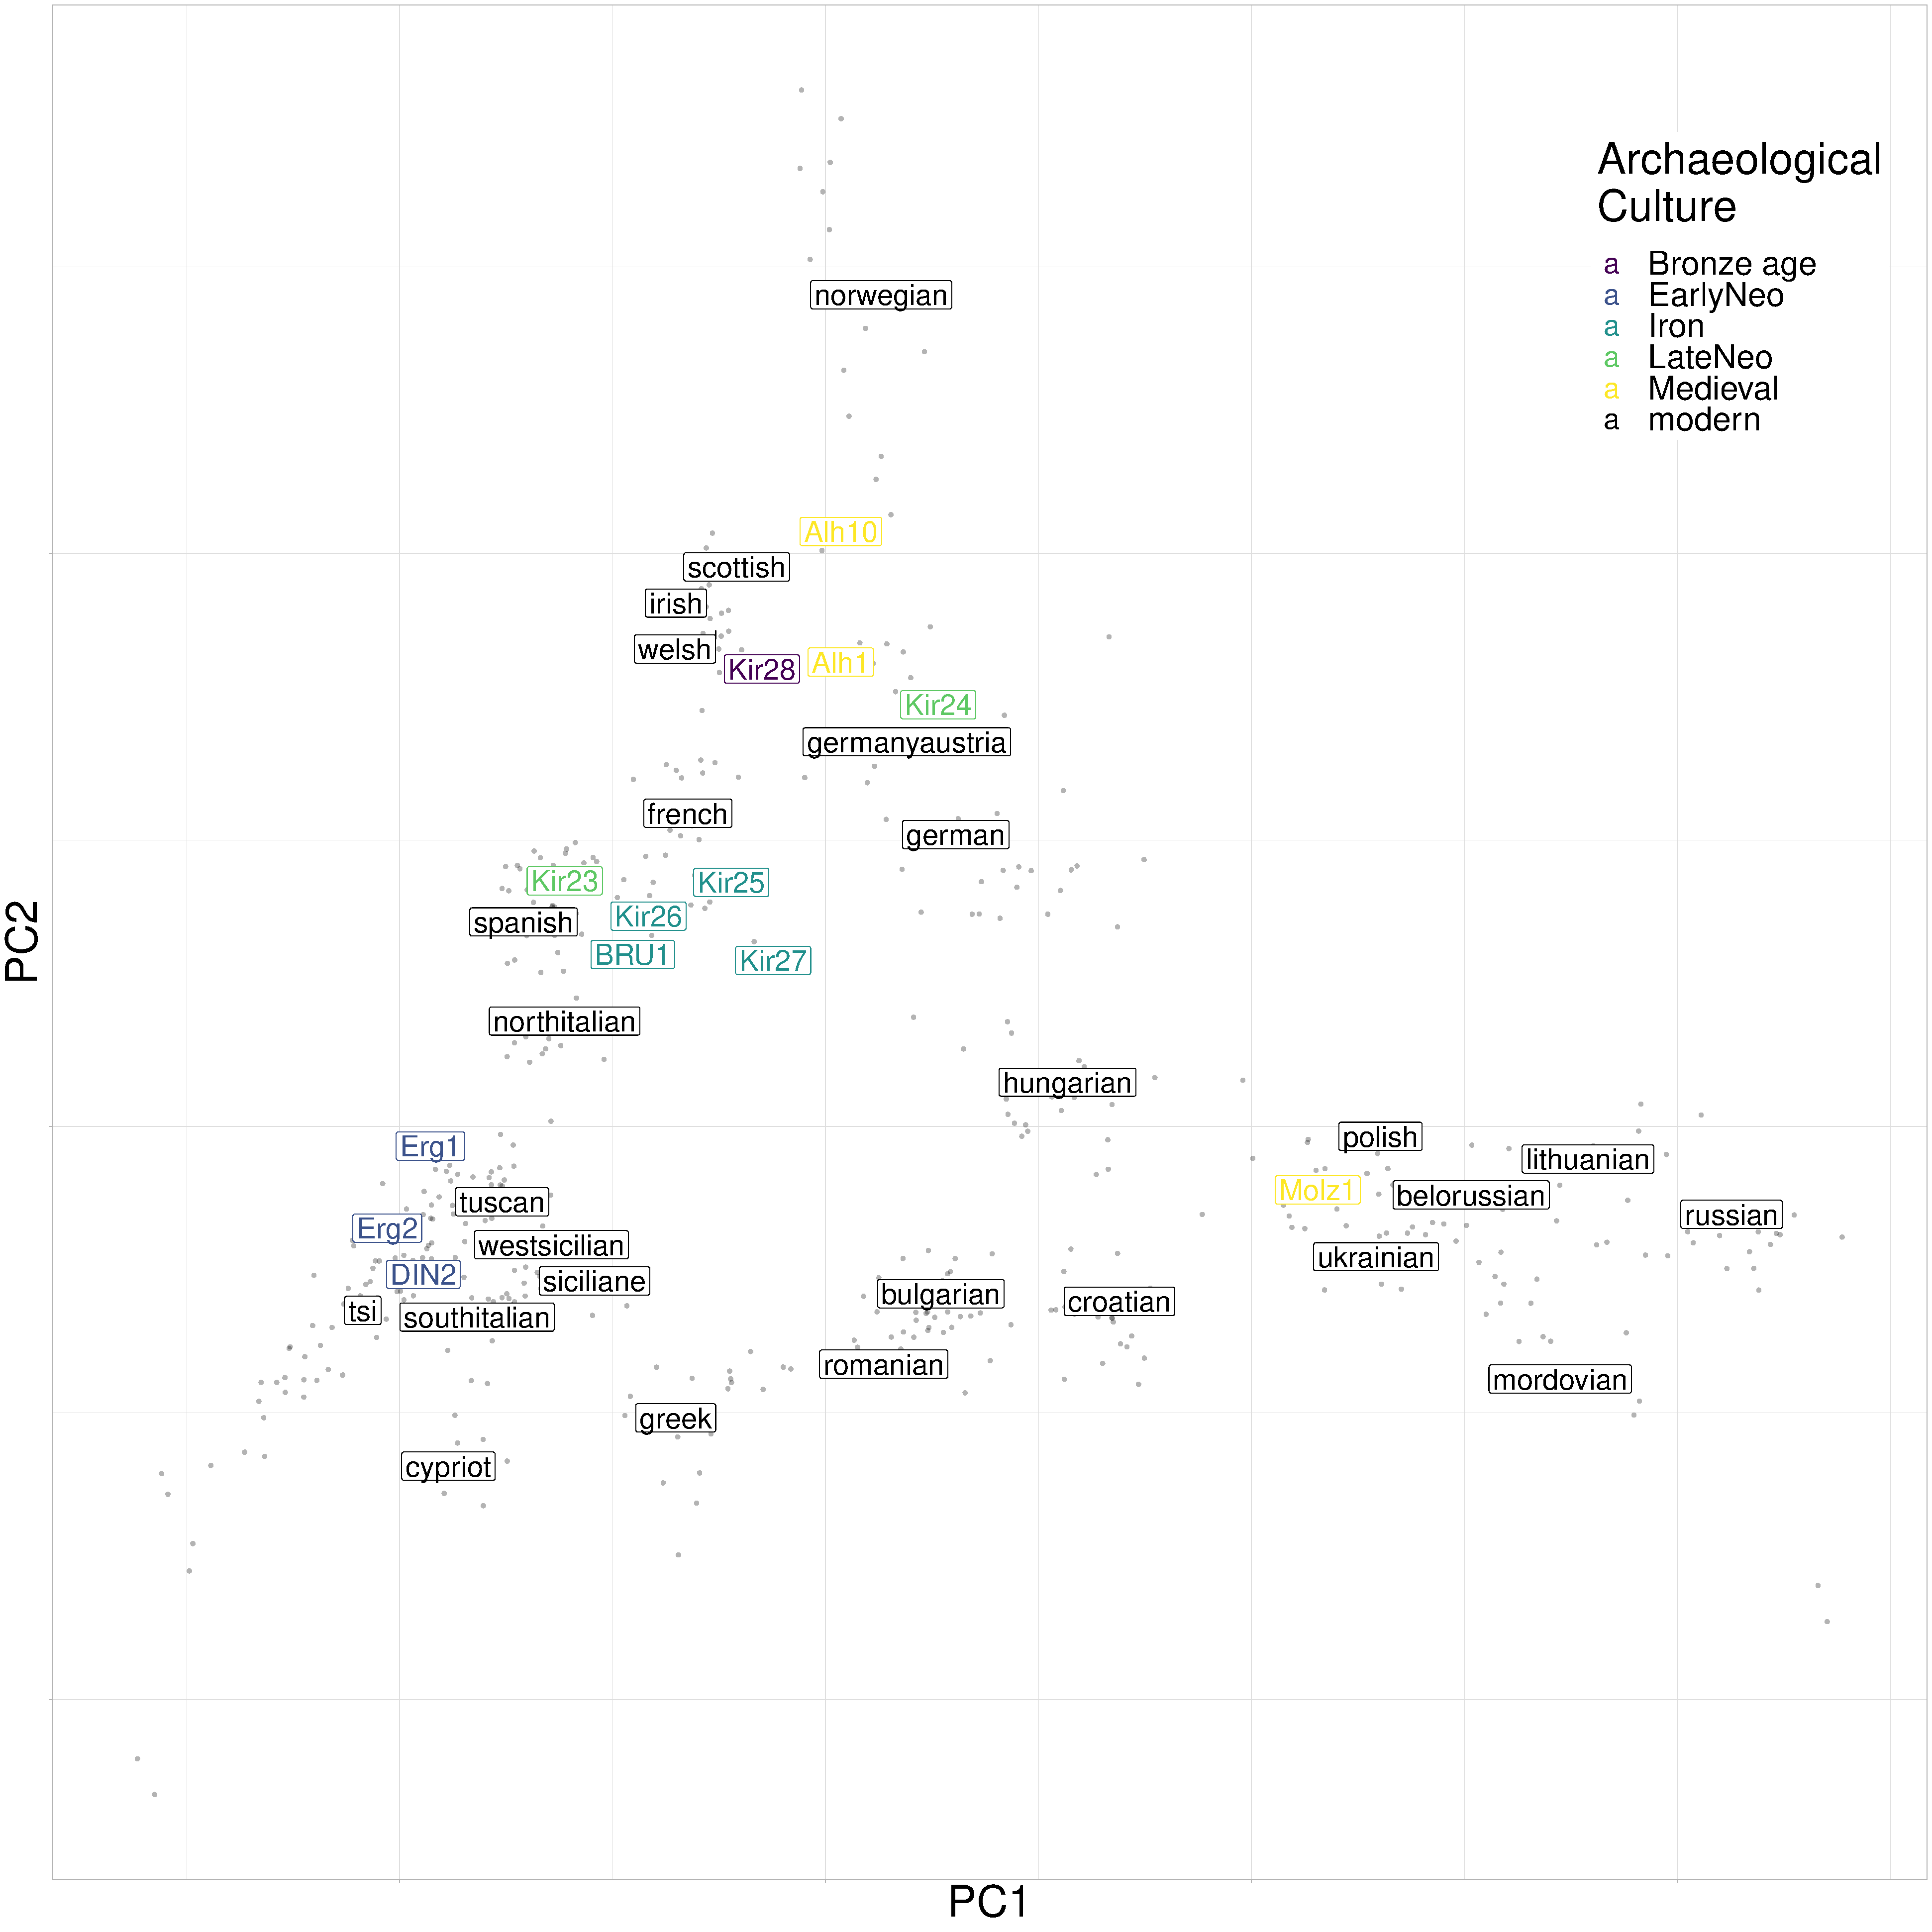
\includegraphics[width=1.0\textwidth]{../images/chapter4/chunklengths_moderns_ancients_PCA.pdf}
    \caption{Principle component plot of newly sequenced ancient samples and reference modern individuals performed using the finestructure library. Green labels correspond to Migration Era samples, red labels correspond to Early Middle Age samples and white labels correspond to reference populations. The position of each reference label is the mean PC coordinates of all individuals within that population. Transparent coloured points correspond to present-day individuals.}
    \label{fig:chunklengths_moderns_ancients_PCA}
\end{figure}

The 3 Early-Middle Neolithic samples all display strong affinity to Anatolian farmers, consistent with the prevailing theory that near-eastern farmers were responsible for the spread of farming across Europe, and that all Neolithic farmers share recent common ancestry \cite{Haak2010, haak2005ancient, bramanti2009genetic, Lazaridis2014}. fineSTRUCTURE analysis grouped Erg1 with 2 samples from Upper Paleolithic/Neolithic Italy and DIN2 clusters with Neolithic samples from Germany, Greece, Anatolia and Hungary. Despite their age, the genetic variation of the Early Neolithic samples falls well within the variation of present-day individuals; when painted using modern individuals, the 3 Early Neolithic individuals cluster with present-day Italians, consistent with previous research \cite{Lazaridis2014, Haak2015} (Fig. \ref{fig:chunklengths_moderns_ancients_PCA}). Erg1 was assigned to mtDNA haplogroup K which has been found in Neolithic and pre-pottery sites across Europe \cite{Hofmanova2016, fernandez2014ancient} and Western Asia \cite{Lazaridis2016, Mathieson2015}. 

Erg1 is from the \textit{Linearbandkeramik} (LBK) culture and is speculated to have belonged to the first wave of immigrants carrying farming technology from south-eastern Europe or Anatolia into central Europe. DIN2 is from a nearby site and around 500 years more recent, and is thought to potentially belong to a second wave of farmers who migrated along the Danube (J. Burger 2018, personal communication). It is unclear to what extent these different waves corresponded to populations with different ancestries.  

When painted using 465 ancient samples from the literature and the newly sequenced samples, Erg1 had the lowest $TVD$ with DIN2, supporting the hypothesis that they were from the same source population. It had the second lowest $TVD$ with Ess7, another LBK sample, from Essenbach, Germany. DIN2 also shares low $TVD$ with Ess7, but has the lowest $TVD$ with NE5 and NE7, samples assigned to Middle and Late Neolithic cultures on the Hungarian plane. DIN2 was assigned to mitochondrial haplogroup J1C, the same as the samples NE4 and NE5. Both the autosomal and mtDNA link to Neolithic Hungary supports the hypothesis that DIN2 migrated along the Danbian route.   

To explicitly test whether Erg1 and DIN2 group together to the exclusion of other ancient samples and therefore, whether they likely originated from a similar source population, I performed $f_{4}$ tests in the form of $f_{4}(W=Erg1, X=DIN2; Y=test, Z=Mbuti)$, where $test$ is 143 ancient populations used in the F-statistics analysis. This tests whether Erg1 and DIN2 form a clade to the exclusion of $test$ or not. Of the 143 comparisons, only the population labeled as WHG had a $|Z|>3$, ($Z=3.057$), suggesting that Erg1 and DIN2 originate from the same local population. However, this result was surprising given we would not typically expect an individual from the LBK culture to form a clade with hunter-gatherer populations. However, this could be indicative of gene flow between a WHG-like source and Erg1. This result was robust to outgroup choice.  

To determine whether Erg1 showed increased genetic similarity to local farming populations, I also performed combinations of $f_{3}$ in the form of $f_{3}(A=Erg1, B=test, C=Mbuti)$, where $test$ iterates across 143 ancient populations. This tests the branch length, or the amount of genetic drift that has occurred on the branch between Erg1 and $test$ since their divergence from an outgroup. The sample/population with the highest $f_{3}$ statistic was NE7, a sample from 4,360 – 4,490 BC and the Lengyel culture (a Neolithic culture centered on the Danube River, known to be an offshoot of the LBK culture Erg1 belonged to). On the other hand, DIN2 shows a clear affinity to samples from neolithic France.

I obtained SNP-capture data from several other local LBK populations; samples from Schwetzingen, Stuttgart-Mullhausen and Halberstadt (Rivollat samples). These samples appear to form a distinct cluster on the unlinked PCA and are shifted away from the primary cluster of Neolithic individuals and towards samples from the Anatolian Bronze Age and Baden Culture (a central European Chalcolithic culture). I wanted to know which LBK population Erg1 and DIN2 were closest to. I found strong evidence ($|Z| = 7.97$) that Erg1 shared mored alleles with LBK populations from Schwetzingen than with Stuttgart-Mühlhausen, suggesting the early LBK populations showed relatively fine-scale geographic structure. Given the lack of Hunter Gatherer ancestry in the Rivollat LBK samples, this structure seems unlikely to be driven by variable amounts of Hunter-Gatherer admixture (Fig. \ref{fig:HG_ancestry_Neolithic}).

\begin{figure}[htp]
    \centering
    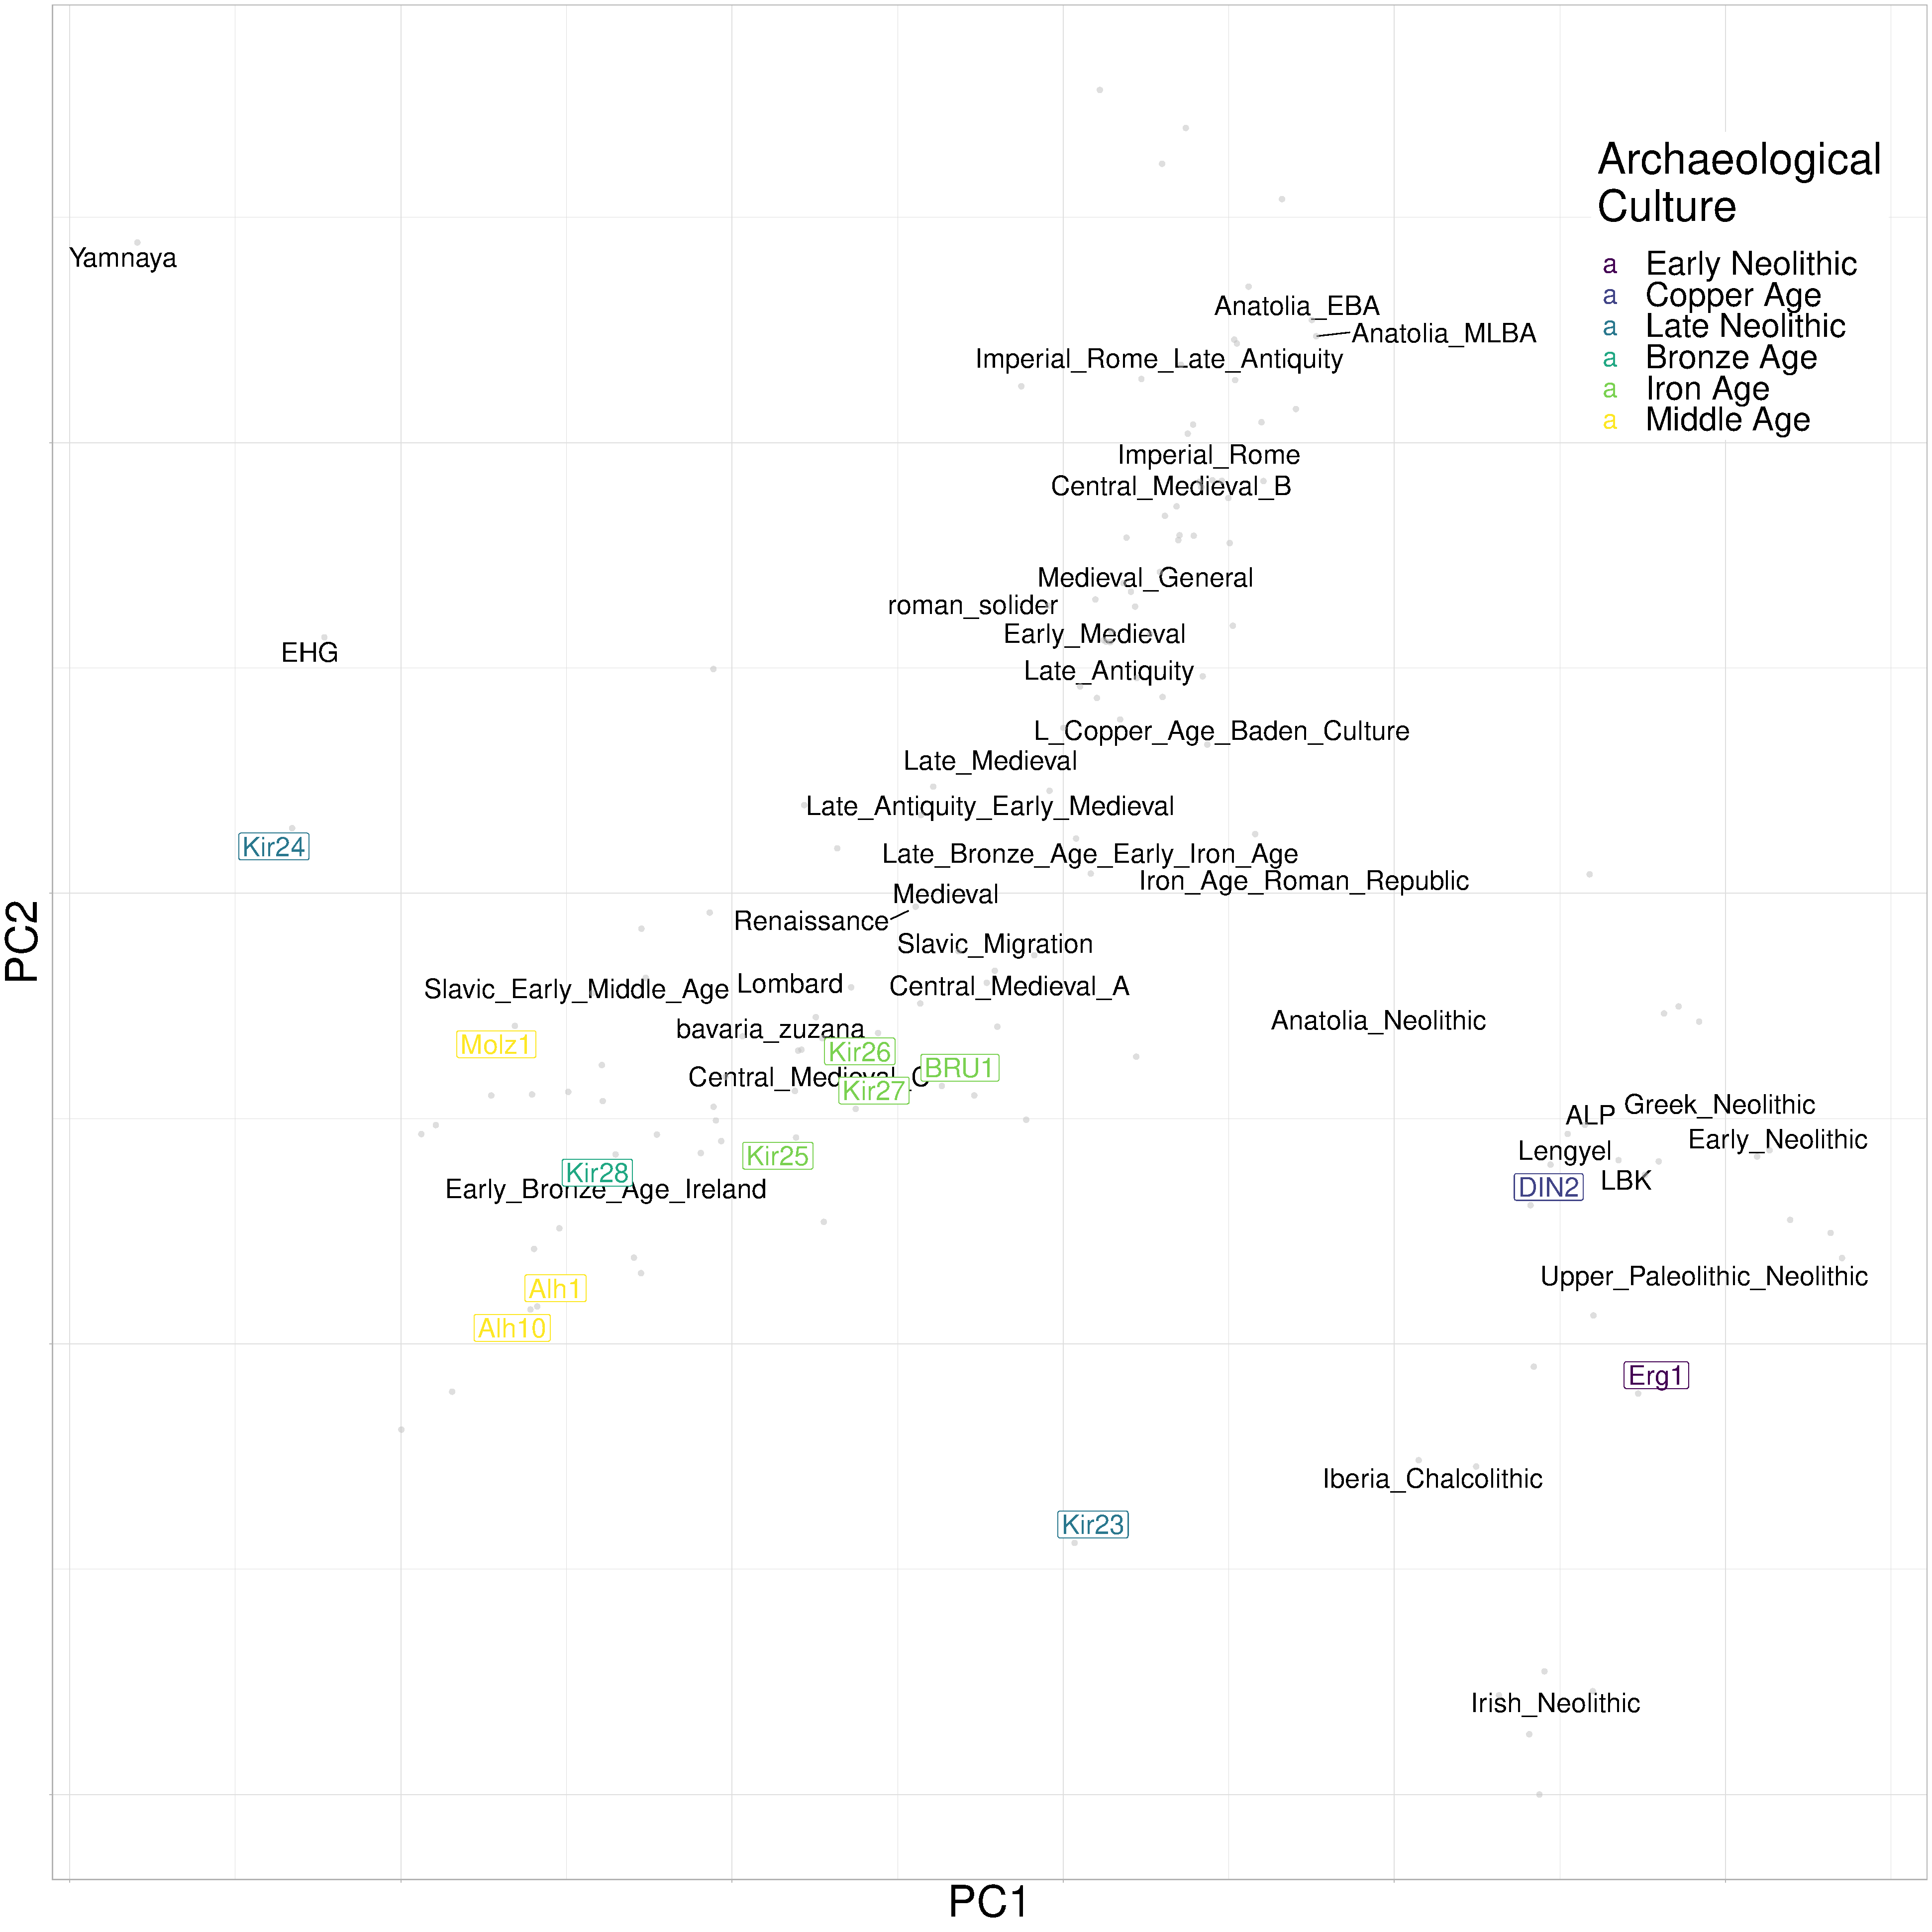
\includegraphics[width=1.0\textwidth]{../images/chapter4/chromopainter_PCA.pdf}
    \caption{Principle component plot of newly sequenced ancient samples and reference ancient individuals performed using the finestructure library. Filled labels correspond to newly sequenced individuals and white labels correspond to reference populations. The position of each reference label is the mean PC coordinates of all individuals within that population}
    \label{fig:chapter4_results_finestructure pca}
\end{figure}

\subsection{Hunter-gather ancestry in Neolithic farmers}

Prior research has shown that admixture occurred between newly arrived farming immigrants from Anatolia and local hunter-gatherers \cite{Gamba2014, Lipson2017b}. The position of Erg1 on the PCA suggests that it may have a significant component of Hunter-Gatherer ancestry. I applied the SOURCEFIND algorithm to the `ancients painting' co-ancestry matrix to infer ancestry proportions for all newly sequenced individuals, fixing 3 surrogate populations at WHG, Yamnaya and Anatolian Neolithic (Fig. \ref{fig:plots3PopBarlot}). I inferred 26\% WHG ancestry in Erg1, suggesting it may have had a relatively recent ancestor who was a Hunter-Gatherer. I inferred a smaller proportion of WHG ancestry into DIN2 (8\%), perhaps suggesting that they were part of a structured local population, where different elements received varying amounts of hunter-gatherer admixture. qpAdm modeling broadly agreed with these estimates and showed that Erg1 can be modeled as a mixture of Anatolia Neolithic (61\%, se=0.095) and WHG (0.3855\%, se=0.095). Erg2 showed no evidence of hunter-gatherer ancestry and could be modeled directly as Anatolian Neolithic farmer, again implying it was part of a structured population with differential amounts of hunter-gatherer admixture. 

\begin{figure}[htp]
    \centering
    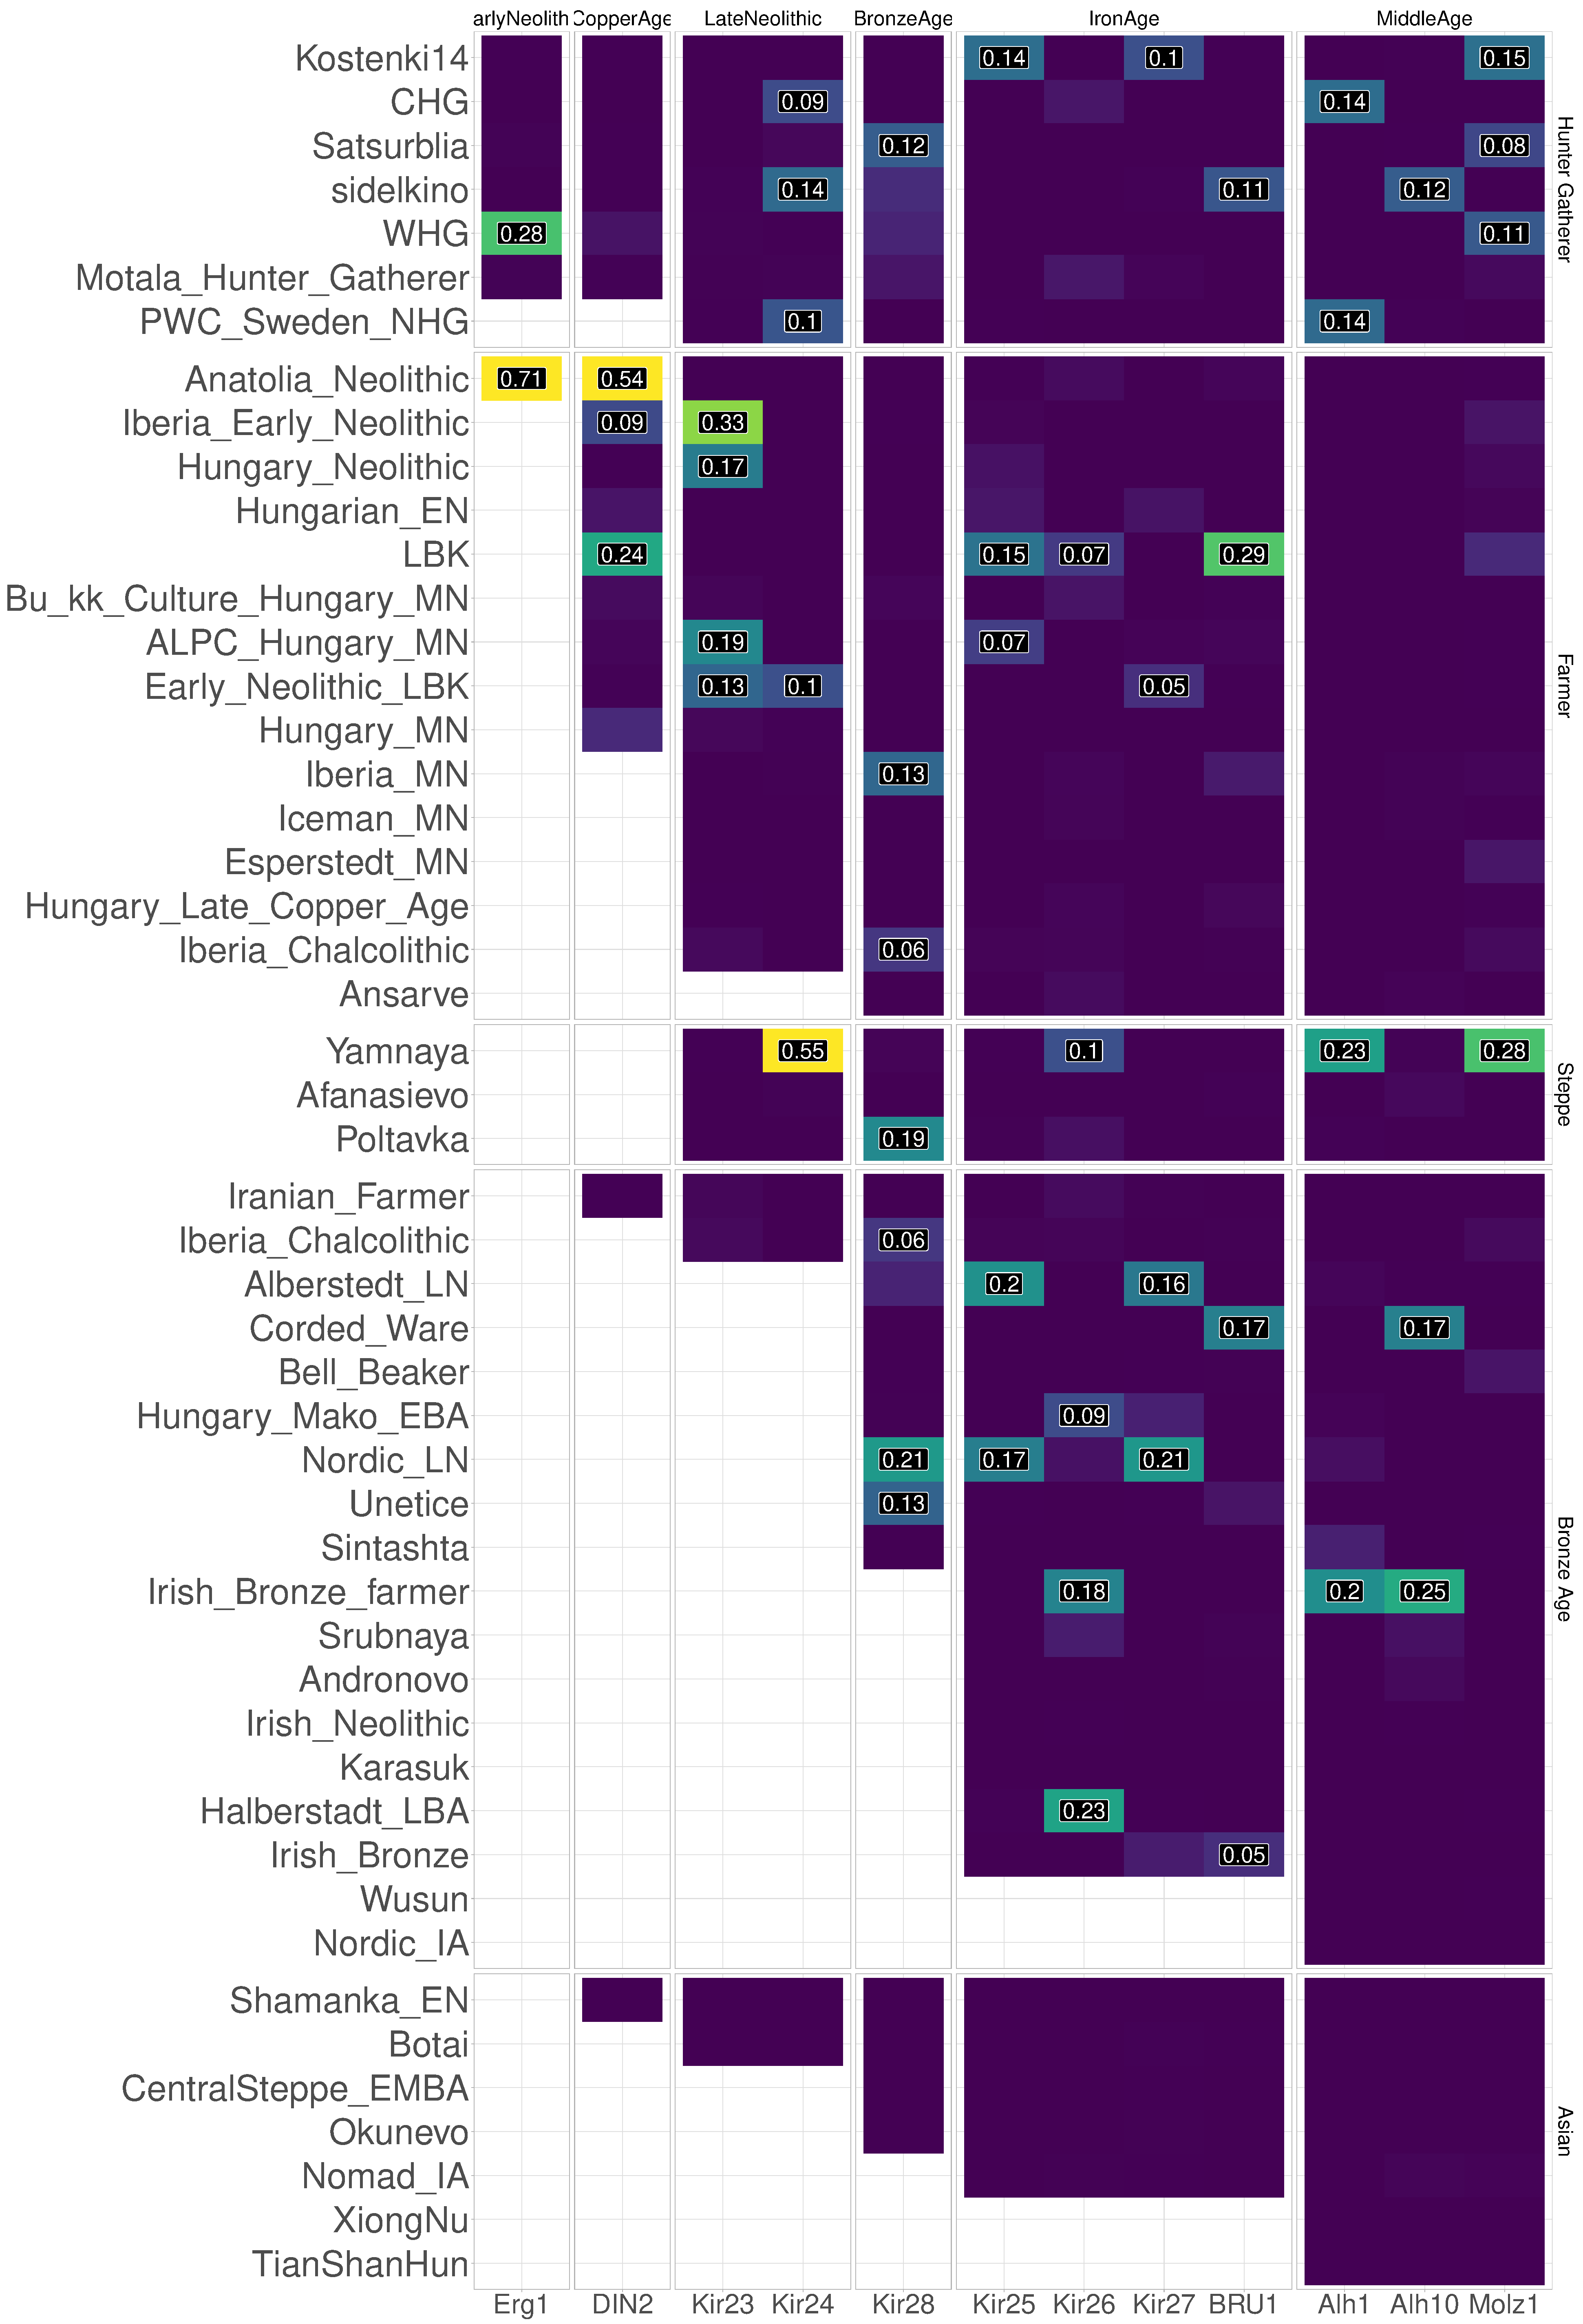
\includegraphics[width=1.0\textwidth]{../images/chapter4/SOURCEFINDheatmapOlderSurrogates_2.pdf}
    \caption{SOURCEFIND ancestry proportion estimates for all newly sequenced target samples (vertical columns). Target samples are grouped by archaeological age. Surrogate populations are represented as horizontal rows and also grouped into archaeological culture. Each target was modeled as a mixture of only populations which are dated to being older or contemporaneous as the the target. Numbers within each cell correspond to the ancestry proportion estimate.}
    \label{fig:chapter4resultsSFheatmapolder}
\end{figure}

To localise the closest source of Hunter-Gatherer admixture into Erg1, I re-performed the 3-population SOURCEFIND analysis, but instead split up the WHG surrogates into Loschbour, LaBrana, Bichon and the 2 individuals from the Iron Gates, leaving 6 surrogate populations in total. I inferred that the two 8800-year-old Iron Gates individuals from Serbia contributed towards 33\% of the ancestry of Erg1, showing that it was likely to be closest population to the mixing source in our dataset. To confirm that this was not an artefact of there being 2 Iron Gates individuals (where all of the other WHG populations had a single sample), I removed the lowest coverage Iron Gates individual from the surrogate pool and repeated the analysis. The proportion of ancestry inferred from Iron Gates was similar (31\%), suggesting the sampling did not affect the inferred proportion.

To determine the date of admixture between an Anatolian Farmer-like and WHG-like source into Erg1, I used MOSAIC \cite{MOSAIC_2019}, which infers admixture events using a similar technique to chromosome painting. MOSAIC is able to model the `true' admixing sources and determine the genetic differentiation between those and the sampled sources, in addition to the date of admixture. When modeled as a 2-way admixture event, MOSAIC inferred similar WHG and Anatolia Neolithic mixing proportions to SOURCEFIND. It inferred the cluster of Italian hunter-gatherers to be the closest population to the true mixing source (Fig. \ref{fig:Erg1_MU_matrix}). MOSAIC is able to infer the Fst between the `true' mixing groups and the sampled populations. I inferred very low Fst between the true and source populations, suggesting we had sampled a good proxy for the `true’ mixing sources. I inferred an admixture date of 5.3 generations before the Erg1 was alive. I caution that the admixture date may be unreliable due to only targeting a single individual and given MOSAIC boostraps over individuals (rather than over Chromosomes as in GLOBETROTTER or LD blocks as in qpAdm), it was not possible to obtain confidence intervals around admixture date. 

\begin{figure}[htp]
    \centering
    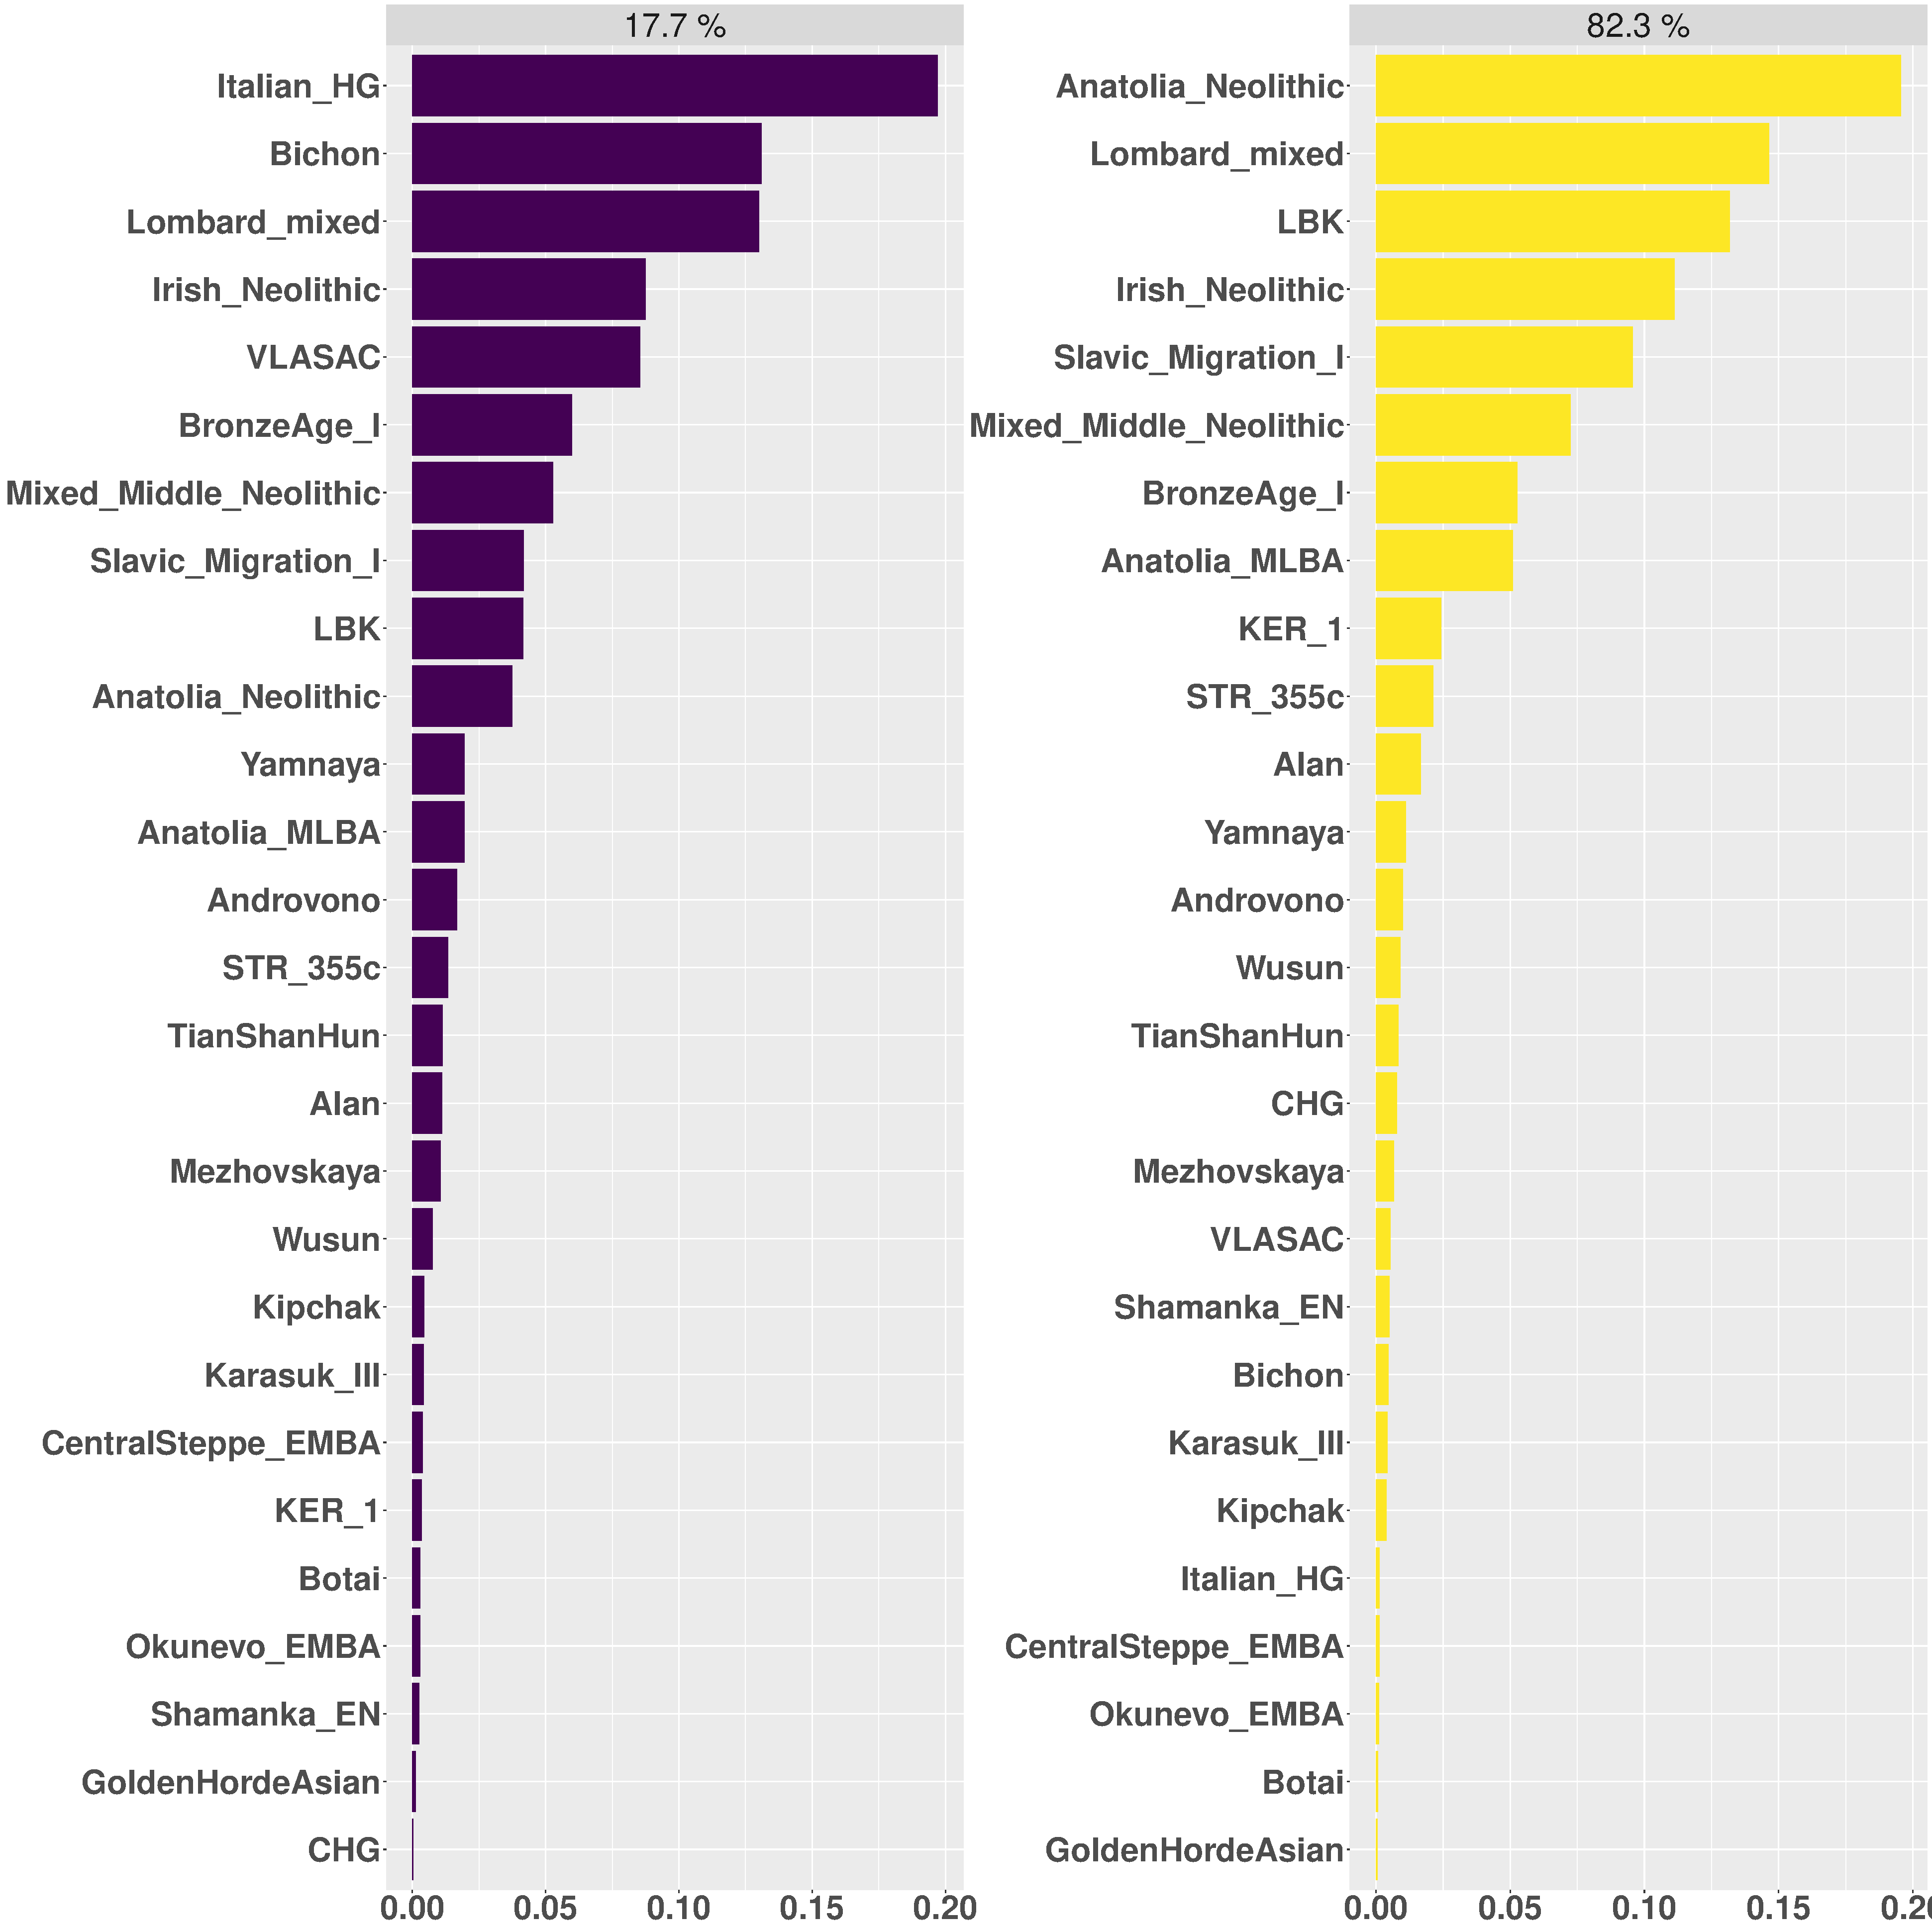
\includegraphics[width=1.0\textwidth]{../images/chapter4/Erg1_MU_matrix.pdf}
    \caption{Copying matrix plot for sources in 2-way admixture event for Erg1. Each panel represents one of the 2 mixing sources. Labels above each panel gives the proportion that mixing source contributed to the Early Middle Age samples. Length of the bars within each panel represent the amount that mixing source copied from a particular population.}
    \label{fig:Erg1_MU_matrix}
\end{figure}

To confirm this admixture event, I performed an $f_{3}$ admixture test, which, when significantly negative, provides unambiguous evidence of an admixture event \cite{Patterson2012}. I performed the test $f_{3}(A=Castelnovian\_Mesolithic, B=Anatolia\_Neolithic, C=Erg1)$, selecting the A and B populations as those were inferred by MOSAIC to be closest to the admixture sources. This did not yield a significant result $(Z=1.96)$. However, exchanging Anatolia\_Neolithic for LBK, a source temporally and geographically more proximate to Erg1 yielded a significant result $(Z=4.25)$. 

I also obtained SNP-capture data from several other local LBK populations; samples from Schwetzingen, Stuttgart-Mullhausen and Halberstadt (Rivollat samples). These samples appear to form a distinct cluster on the unlinked PCA and are shifted away from the primary cluster of Neolithic individuals and towards samples from the Anatolian Bronze Age and Baden Culture (a central European Chalcolithic culture) (Fig. \ref{fig:plink_PCA}). I wanted to contextualise the amount of Hunter-Gatherer in the newly sequenced samples, compared to different French and German farmer groups. As expected, and shown by previous studies \cite{Lipson2017}, Early Neolithic populations show little sign of Hunter-Gatherer ancestry, which appears more into the Middle Neolithic and further west from Greece and Anatolia. Populations from France, in particular early samples, show the highest amount of HG ancestry. However, contemporaneous populations from Germany display much reduced levels of HG ancestry and can fit a model of purely Anatolia Neolithic ancestry well. Our sample Erg1 appears to be an exception, displaying high levels of HG ancestry comparable to the samples found in France (Fig. \ref{fig:HG_ancestry_Neolithic}). On the other hand, Erg2, a sample which is contemporaneous and local to Erg1, showed no evidence of Hunter Gatherer admixture 

\begin{figure}[htp]
    \centering
    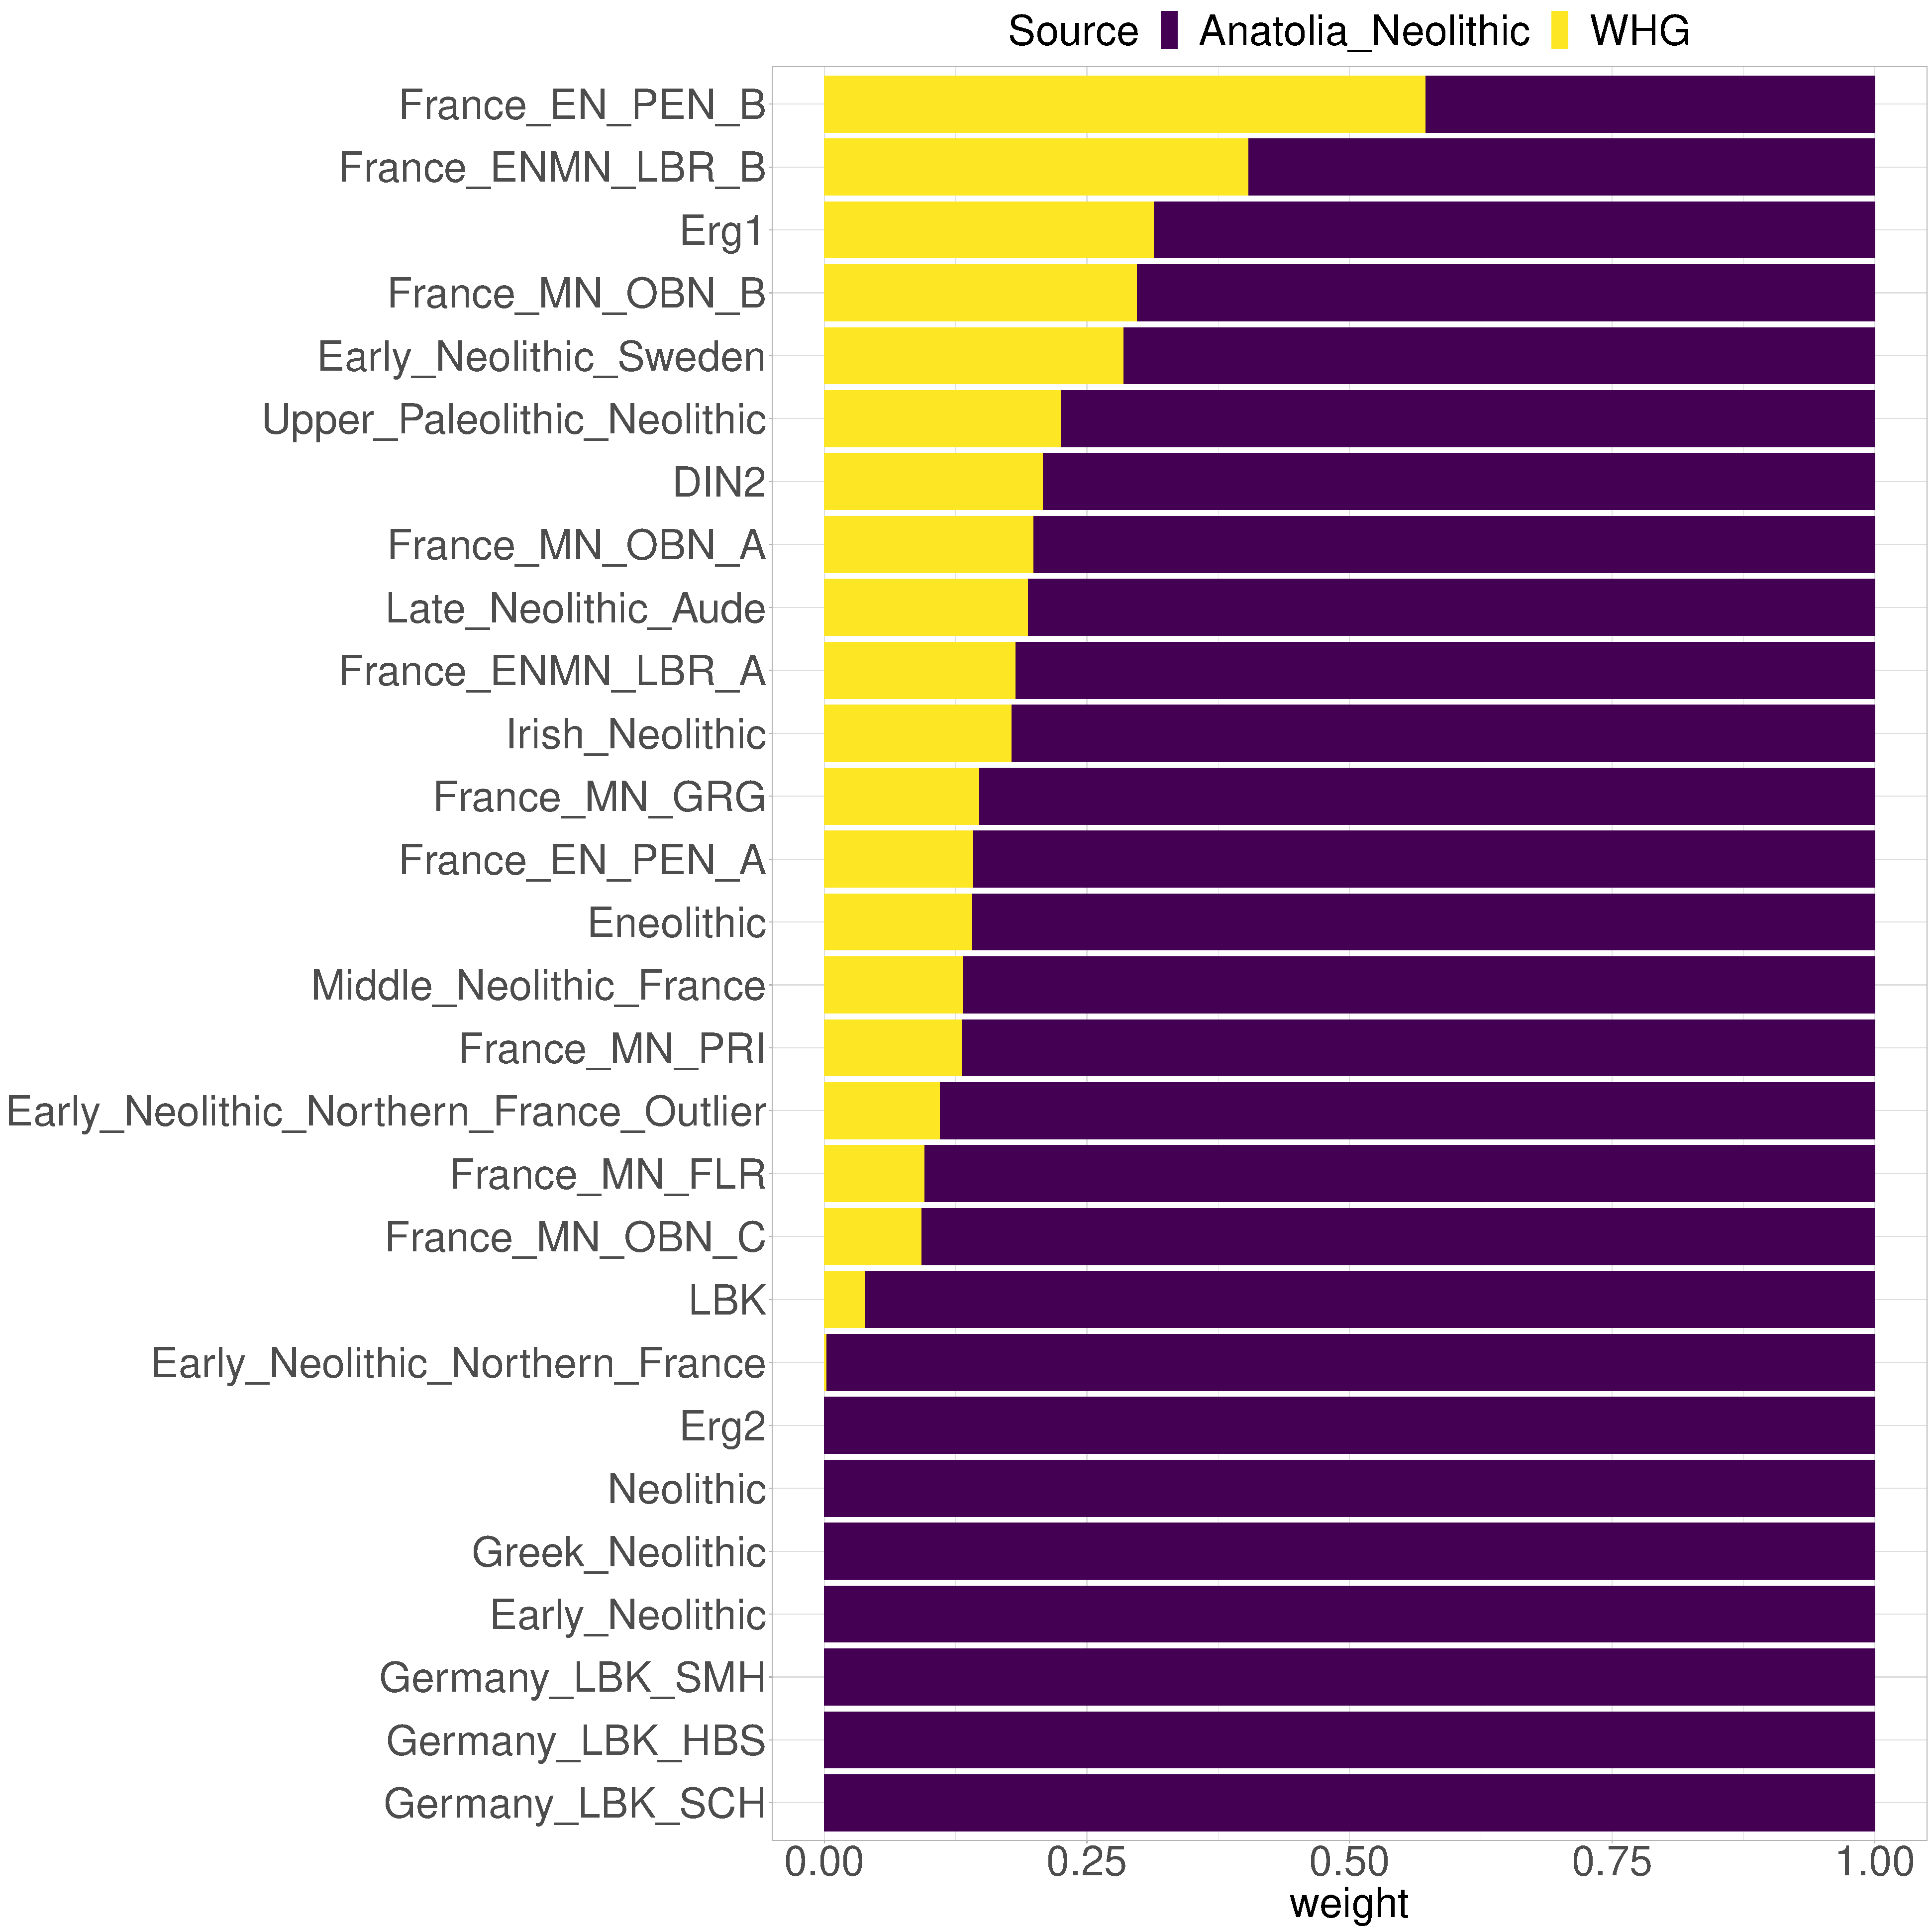
\includegraphics[width=1.0\textwidth]{../images/chapter4/HG_ancestry_Neolithic.pdf}
    \caption{qpAdm ancestry proportion estimates for a selection of European Neolithic individuals. All individuals were modeled as a 2-way mixture between Anatolian Neolithic farmers and Western-Hunter Gatherers (WHG). Outgroups given in methods 4.2.9.}
    \label{fig:HG_ancestry_Neolithic}
\end{figure}


\begin{figure}[htp]
    \centering
    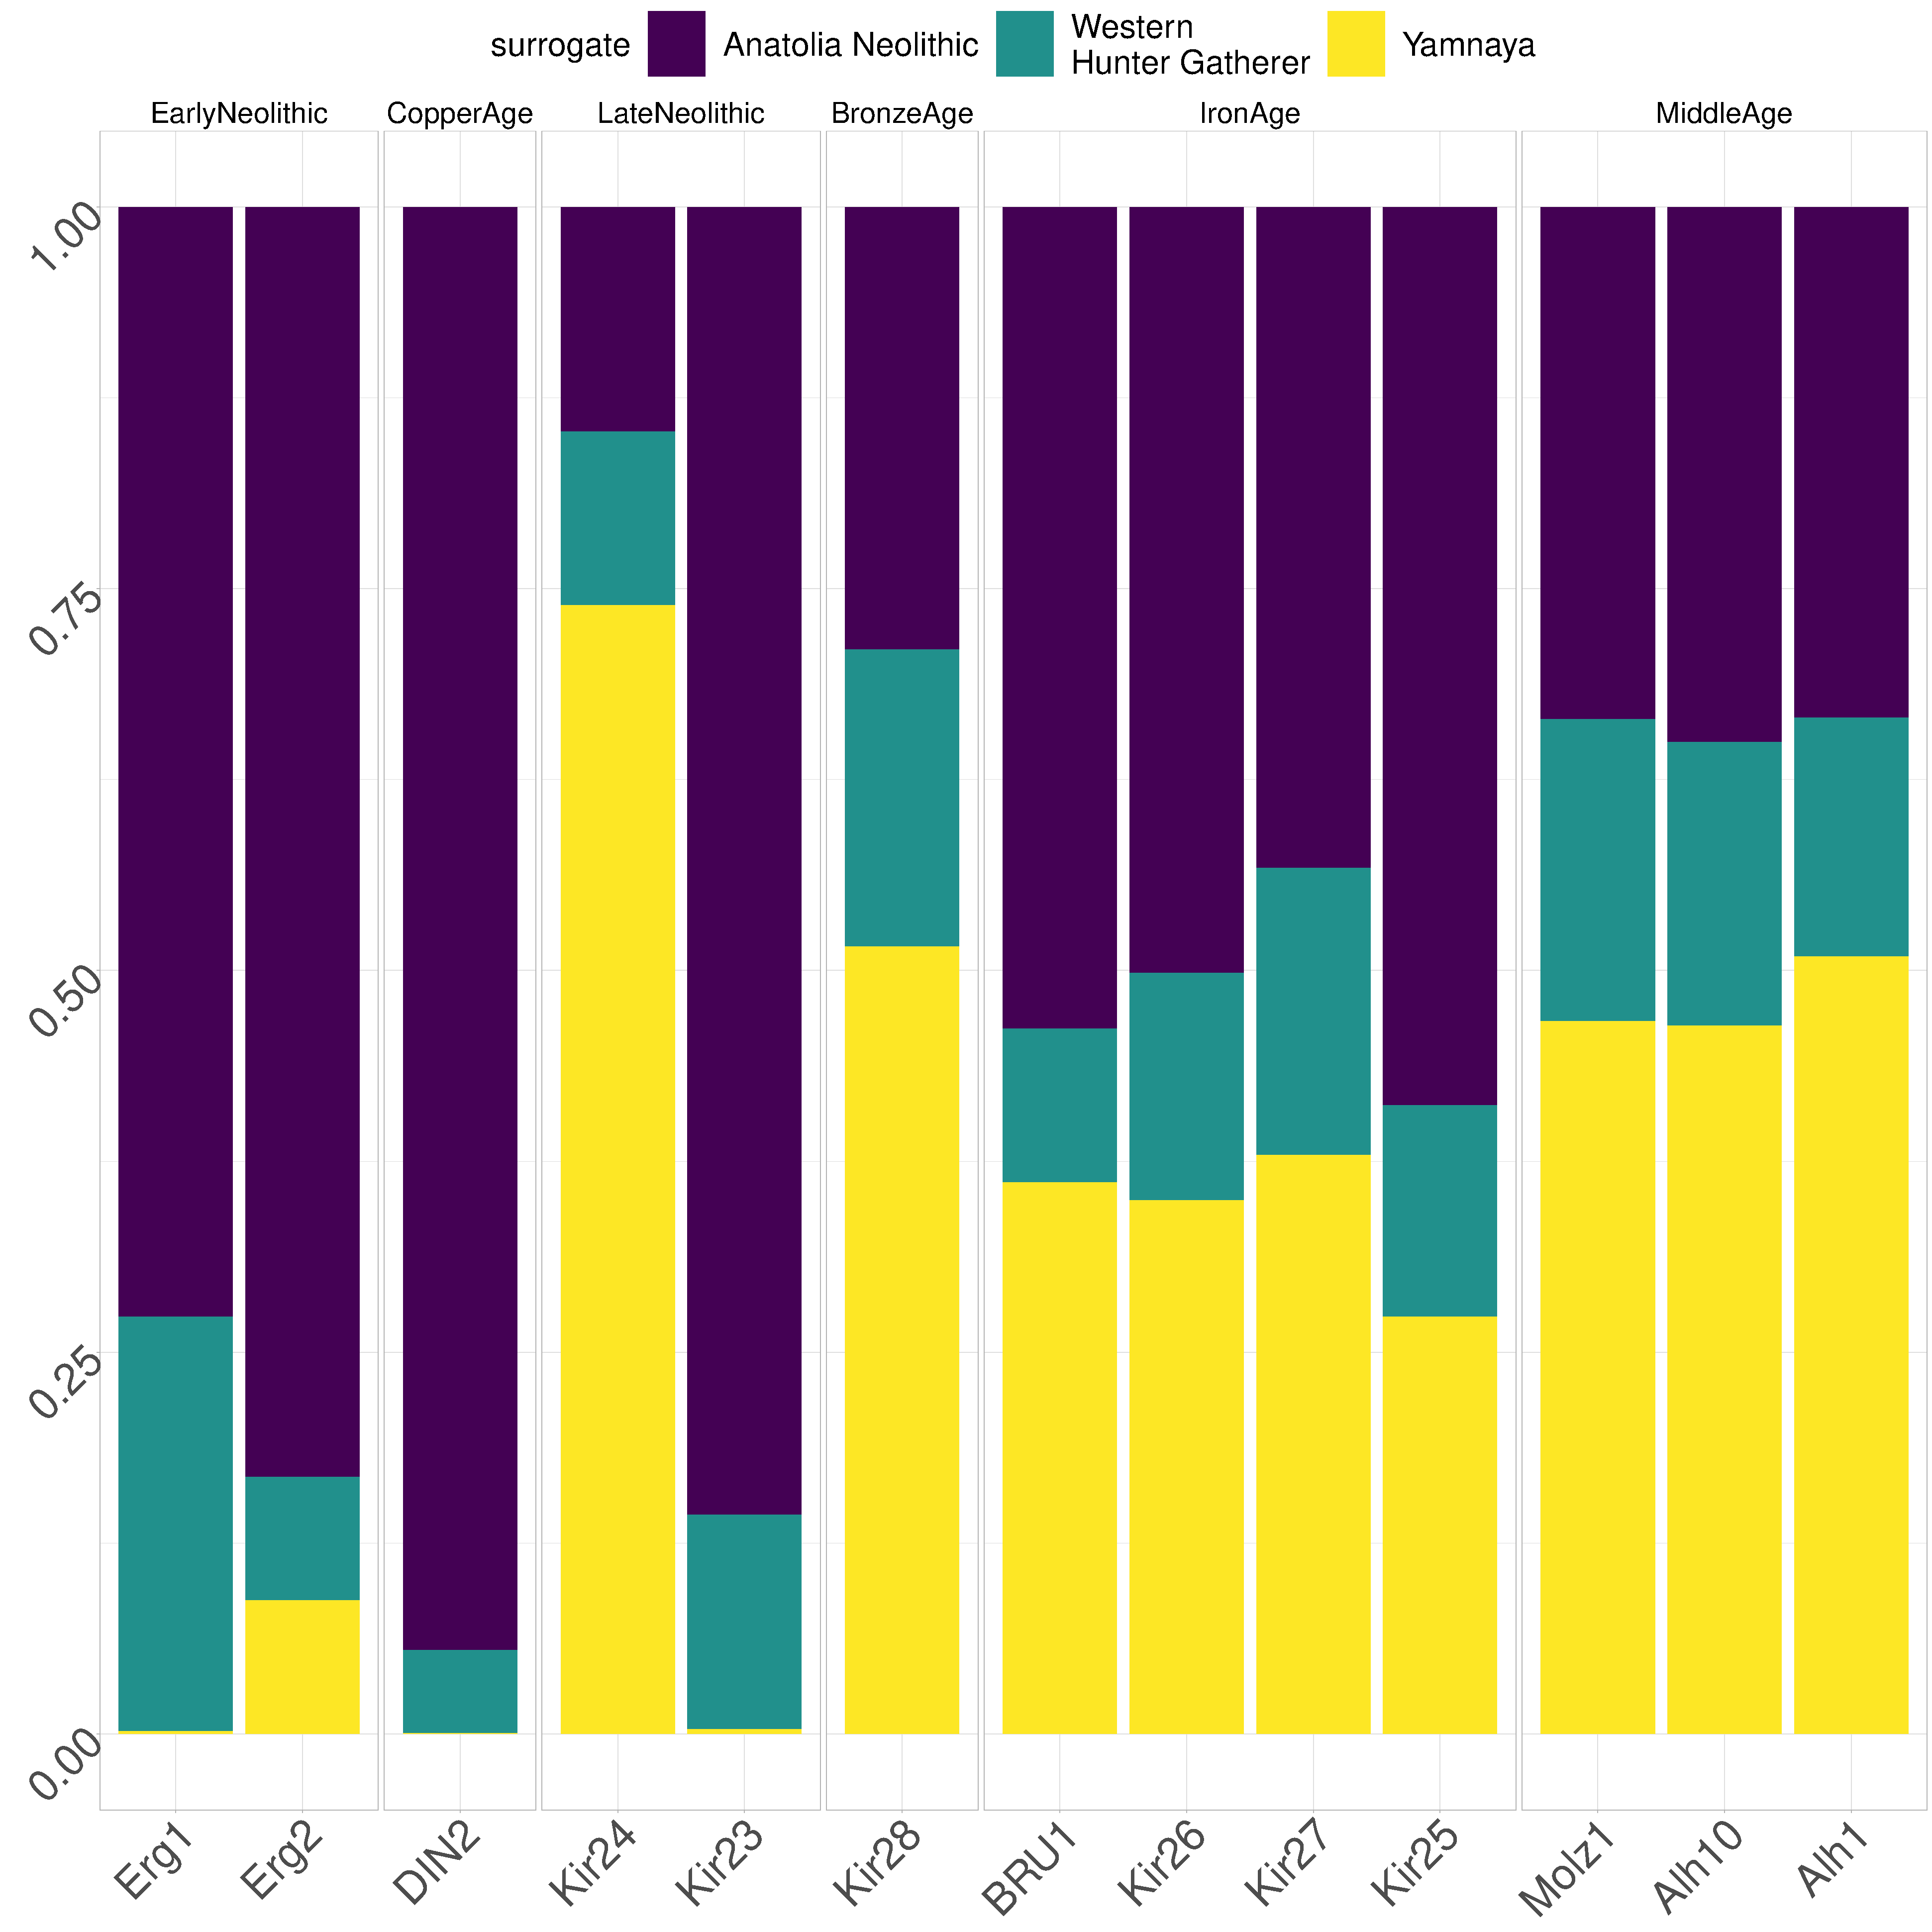
\includegraphics[width=1.0\textwidth]{../images/chapter4/plots3PopBarlot.pdf}
    \caption{SOURCEFIND ancestry proportion estimates for all newly sequenced target samples (vertical columns). Target samples are grouped by archaeological age. Surrogate populations are represented as horizontal rows and also grouped into archaeological culture. Each target was modeled as a mixture of only populations which are dated to being older or contemporaneous as the the target. Numbers within each cell correspond to the ancestry proportion estimate.}
    \label{fig:plots3PopBarlot}
\end{figure}

\subsection{Late Neolithic}

This dataset included 2 individuals found in the same stratigraphical layer of Cherry-Tree cave; Kir23 and Kir24 were both dated to the Late Neolithic (approx 4700 BP). Despite their temporal and spatial closeness, they show highly different ancestry profiles (Fig. \ref{fig:plots3PopBarlot}). 

On both the plink and ChromoPainter PCA and fineSTRUCTURE clustering, Kir24 clusters with individuals from populations present around the Eurasian Steppe during the Bronze-Age, such as those from the Yamnaya and Afanasievo cultures. These are the populations known to be responsible for the spread of Indo-European languages across Europe \cite{Haak2015}. These results support the findings of Allentoft (2015), who concluded that the Afanasievo Culture were `genetically indistinguishable' from the Yamnaya Culture. That the Yamnaya and Afanasievo samples were sampled in Russia suggests that Kir24 may have been a recent migrant from the Eurasian Steppe. This is supported by IBD analysis; of all the ancient samples in the dataset Kir24 shares the most IBD (31.12cM) with Yamnaya and the lowest $TVD$ with 2 other members of the Yamnaya population. This timing (Kir24 is dated to approximately 4700 BP) corresponds to some of the earliest appearance of Yamnaya-like ancestry in central Europe \cite{Racimo8989}. Using qpAdm, Kir24 could be modeled as a mixture of Yamnaya (93\%, se=12\%) and WHG (6\%, se=8\%) without any Neolithic ancestry. 

Kir24 was assigned to mtDNA haplogroup T1a1, which has been found in Yamnaya samples from the Middle Volga region and Bulgaria \cite{keyser2009ancient}. Additionally, they found the frequency of T1a1 to be higher in the Yamnaya peoples than in any other ancient or modern population. 

On the other hand, Kir23 is found in a fineSTRUCTURE cluster with Ballynahatty, from Neolithic Ireland (3343-3020 BC), and is positioned on both plink and ChromoPainter PCAs with other late Neolithic samples. It is found in adjacent fineSTRUCTURE groups to samples from Neolithic Spain and Ireland. As is the case with other Neolithic samples of this era, Kir23 has a component of Hunter-Gatherer ancestry; it is known that Middle Neolithic individuals are characterised by admixture with the existing Hunter-Gatherer populations. qpAdm modeling showed that Kir23 could be formed from a mixture of Neolithic Anatolia (96\%, se=14)  and Hunter Gatherer (6.25, se=0.91) without the need for additional Steppe ancestry. 

To test whether the source of Neolithic ancestry in Kir23 was most similar to local populations, I performed $f_{4}$ tests in the form $f_{4}(W=Kir23, X=mbutipygy; Y=test, Z=Erg2)$, which tests whether Kir23 forms a clade with Erg2, a local farmer individual, or $test$, where $test$ was one of several different farmer populations. Erg2 was chosen as the local group because it lacked any potentially confounding Hunter Gather ancestry. Kir23 always formed a clade with Erg2, suggesting that the source of ancestry into Kir23 was local and that there was a degree of continuity within the region. 

\subsection{Bronze Age}

The single  Bronze Age individual, Kir28, is dated to approximately 4000BC. Kir28 is found in a fineSTRUCTURE group with other Central Europe Bronze Age samples; RISE150, a sample from the contemporaneous Bronze Age Unetice culture and Rathlin1, a sample from  early Bronze Age Ireland. Thus, this sample is typical

qpAdm modeling showed that the Kir28 can be modeled as a mixture of the two previous Late Neolithic samples in roughly equal proportions, or a mixture of Bell Beakers and Irish Neolithic populations. 

\subsection{Iron Age}

Both the plink and ChromoPainter PCAs show that the Iron Age samples appear to be shifted towards the cluster of Neolithic individuals relative to the Bronze Age. The same pattern is also seen in the modern PCA, where the Iron Age samples are shifted substantially towards Spain / Northern Italy relative to the preceding Bronze Age sample which is situated among Northern / Western European populations (Germany, Wales) (Fig. \ref{fig:chunklengths_moderns_ancients_PCA}). Previous studies into the Bronze-Iron Age transition in Western-Europe (France) have shown relative continuity \cite{Brunel12791}. Other studies in Eastern-Central Europe (Hungary) have shown the Bronze-Iron Age transition was accompanied by an increase in Eastern-European ancestry (albeit from a single sample) \cite{Gamba2014}. I was interested to see whether the transition in Bavaria had elements of either of these phenomena. 

To identify the possible source of `southern' ancestry in the Iron Age samples, I formed each of the Bronze Age, Iron Age and Middle Age Bavarian populations as a mixture of all other ancient populations using SOURCEFIND. I detected a component represented by `Renaissance', a population from approximately 1500CE Italy, which contributed towards 26\% of the ancestry to Iron Age individuals, but was found in neither the preceding Bronze Age nor following Middle Age. Thus, Renaissance samples appear to be the closest proxy for the `southern' ancestry source. qpAdm modeling showed that the Iron Age samples can be well formed from a mixture of the preceding Bavarian Bronze age sample and those from either Renaissance Italy, Imperial Rome, Imperial Rome Late Antiquity or `Roman Solider' from Veeramah et al (2018). All other possible sources included with Bronze Age resulted into poorly fitting models. This suggests a model of admixture from populations best represented by those from post Iron-Age Italy. 

To determine whether this was an admixture event, I grouped the Iron Age samples together and performed MOSAIC admixture analysis. In the 2-way admixture model, the Iron Age samples could be formed of a mixture of a source closest to an Alamannic-Frankish sample (510 – 530 AD) 17.7\% and a source closest to Anatolian Neolithic / LBK samples (82.3\%). The estimated $F_{st}$ between the 2 mixing sources was 0.016, approximately equivalent between present-day Germans and Palestinians \cite{nelis2009genetic}.  Boostrapped dates estimated the date to between 7.86 and 11.31 (95\% quantiles) generations ago. This signal is supported by the fineSTRUCTURE groupings; all 4 Iron Age individuals were grouped alongside several Lombard samples and a Roman solider from 300AD. 

Based on SOURCEFIND modeling with the extended older surrogates set, unlike Gamba et al (2014) \cite{Gamba2014}, I found no evidence of East-Asian or East-Asian-like admixture (Fig. \ref{fig:chapter4resultsSFheatmapolder}).


\subsection{Modern day legacy of the Altheim and Molzbichl samples}

Finally, our dataset included 3 samples from the Middle Age period. The two genomes from Altheim, Germany, date to around 500AD and were found in a Roman context. The single individual from Molzbichl, Austria, dates to around 300 years later, and has been assigned to a `Slavic' context.  

The 3 Middle Age samples appear to share common ancestry based on the plink PCA and are located next to other samples from the Middle Ages. Some structure is apparent from the ChromoPainter PCA, with the two Altheim samples clustering more closely together to the exclusion of the Slavic sample; however, this difference appears to be subtle. $f_{4}$ in the form $f_{4}(mbutipygymy, Bavaria\_Iron; Bavaria\_Slav, Bavaria\_Germanic)$ returned a non-significant result, showing that samples from the Iron Age in Bavaria were symmetrically related to the later Middle Age sample. These results suggest that the differentiation between `Germanic' and `Slavic' populations arose post Iron Age. However this non-significant result could be caused by low sample sizes in the Middle Age populations or a lack of power in allele-frequency based methods.

The two Germanic samples fall into a fineSTRUCTURE cluster with a set of contemporaneous samples from Northern Europe, including 10-11\textsuperscript{th} century Vikings from Estonia, Sweden and Iceland. On the other hand, Molz1 clusters with other individuals known to be from Early Slavic populations. Interestingly, the Slavic cluster also containing a sample DA29, also know as `GoldenHordeEuro'. This sample is from Karasuyr, Kazakhstan, and has was dated to 1200-1400 CE. The Golden Horde was a Mongol khanate established in the 13th Century CE. Given this sample shows clear evidence of European ancestry and clusters alongside individuals from Early Middle Age Europe, it has been proposed that this individual was captured in Europe during the Mongol raids of the 13th Century, when they assaulted the Kievan Rus' federation. That `GoldenHordeEuro' clusters with Molz1 suggests the location of capture in Europe may have been from Austria where Molz1 was found. 

It is currently unknown whether, in addition to cultural and linguistic differences, genetic differentiation exists between the `Germanic’ peoples represented by the two Altheim samples, and the `Slavic’ peoples represented by the Molzbichl sample. All 3 samples are positioned close on the ancients PCA, suggesting they lack differentiation in the context of ancient samples. However, their positions on the modern PCA reveals there was strong differentiation between early Slavic and Germanic peoples (Fig. \ref{fig:chunklengths_moderns_ancients_PCA}). Molz1 clusters with present-day Slavic speaking populations such as Poland, Ukraine and Belarus. On the other hand, the two Germanic samples cluster with present-day individuals from Germanic-speaking countries in Western Europe, such as Scotland, Germany and Wales. 

Plotting differential haplotype sharing between the Slavic and Germanic sample makes this pattern clear (Fig \ref{fig:germanic_slavic_HB_sharing}). There is a clear division down the centre of Europe, dividing it into East and West that shows the structure in present-day Europeans has existed since at least the Early Middle Ages. 

These results were recapitulated using SOURCEFIND, where we modeled each individual as a mixture of different modern-day populations. The two samples from Altheim derived a large proportion of their ancestry to modern day Germans (81.8\%, se=12.8), whereas the Molzbichl sample derived a large proportion of its ancestry from modern day Polish (77.85\%, se=20.3) and Croatians (11.7\%, se=9.1). 

\begin{figure}[htp]
    \centering
    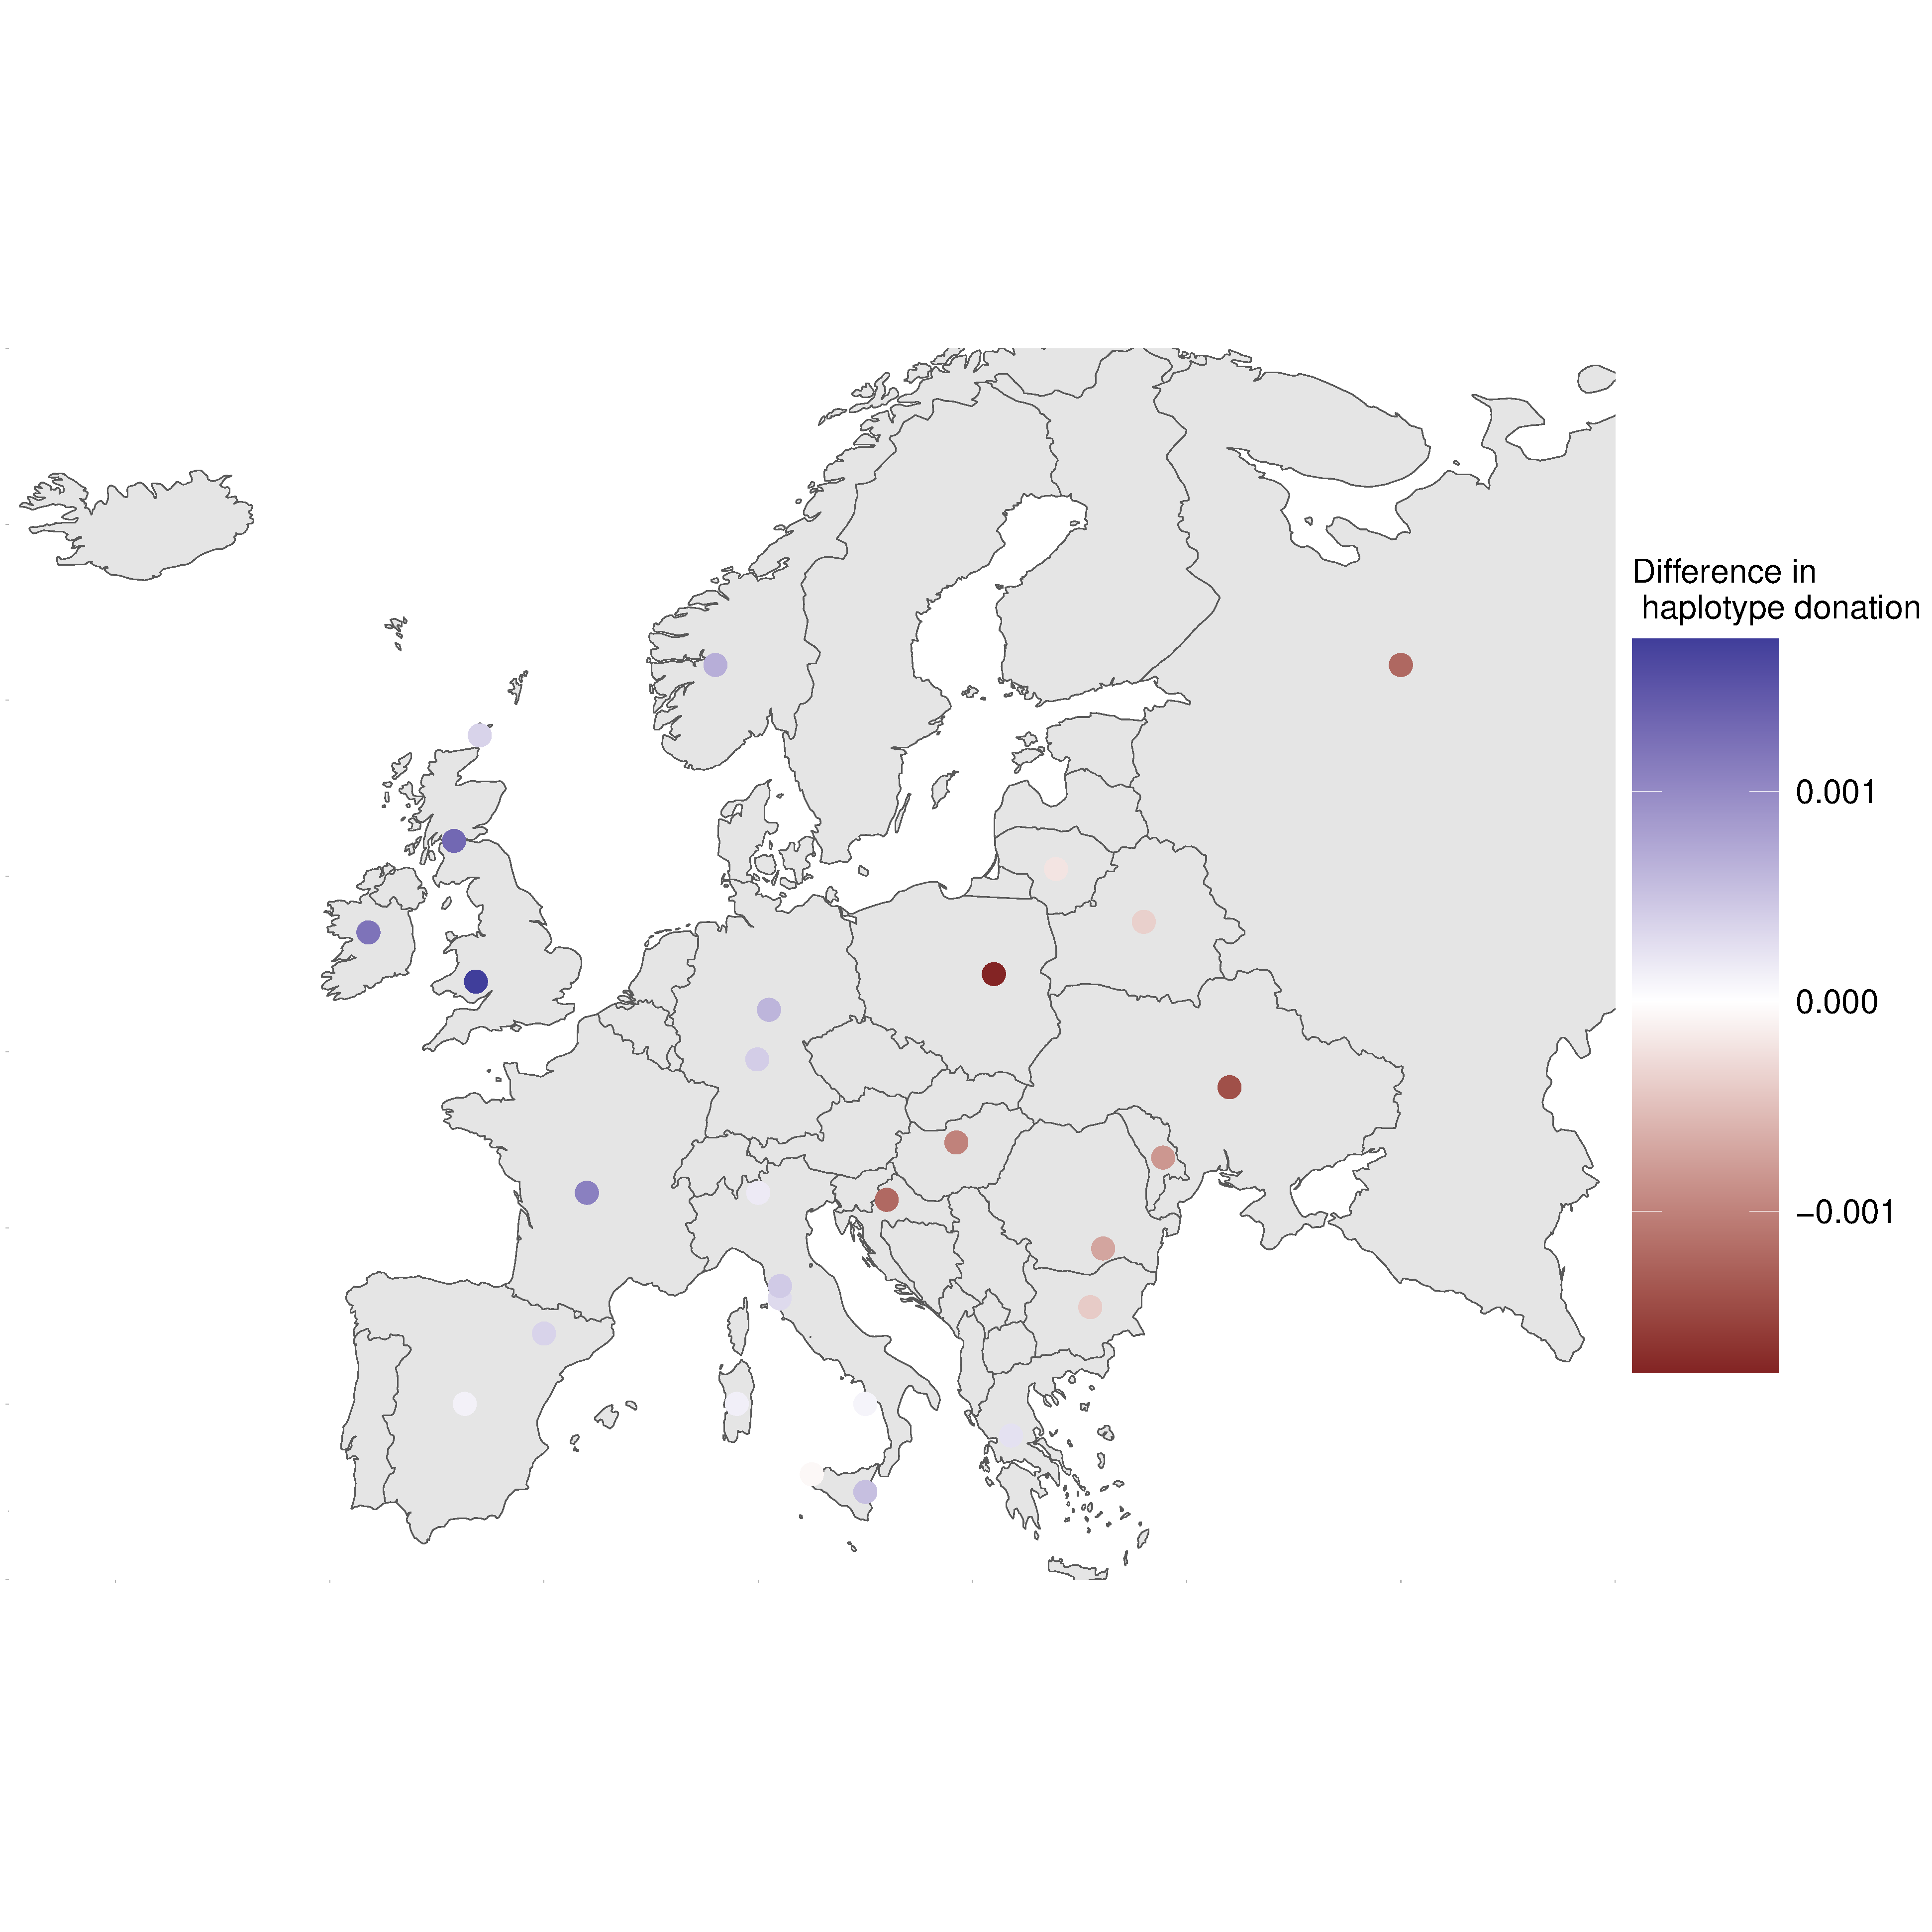
\includegraphics[width=1.0\textwidth]{../images/chapter4/germanic_slavic_HB_sharing.pdf}
    \caption{Differential haplotype-donation between Germanic and Slavic samples. Each coloured point is one present-day population. Points are coloured based on whether they donate relatively more to Germanic (blue) or Slavic (red) ancient samples.}
    \label{fig:germanic_slavic_HB_sharing}
\end{figure}

\subsection{Sample heterozygosity and homozygosity}

I calculated per-sample heterozygosity and runs-of-homozygosity  for all samples above 3x coverage. 

\begin{figure}[htp]
    \centering
    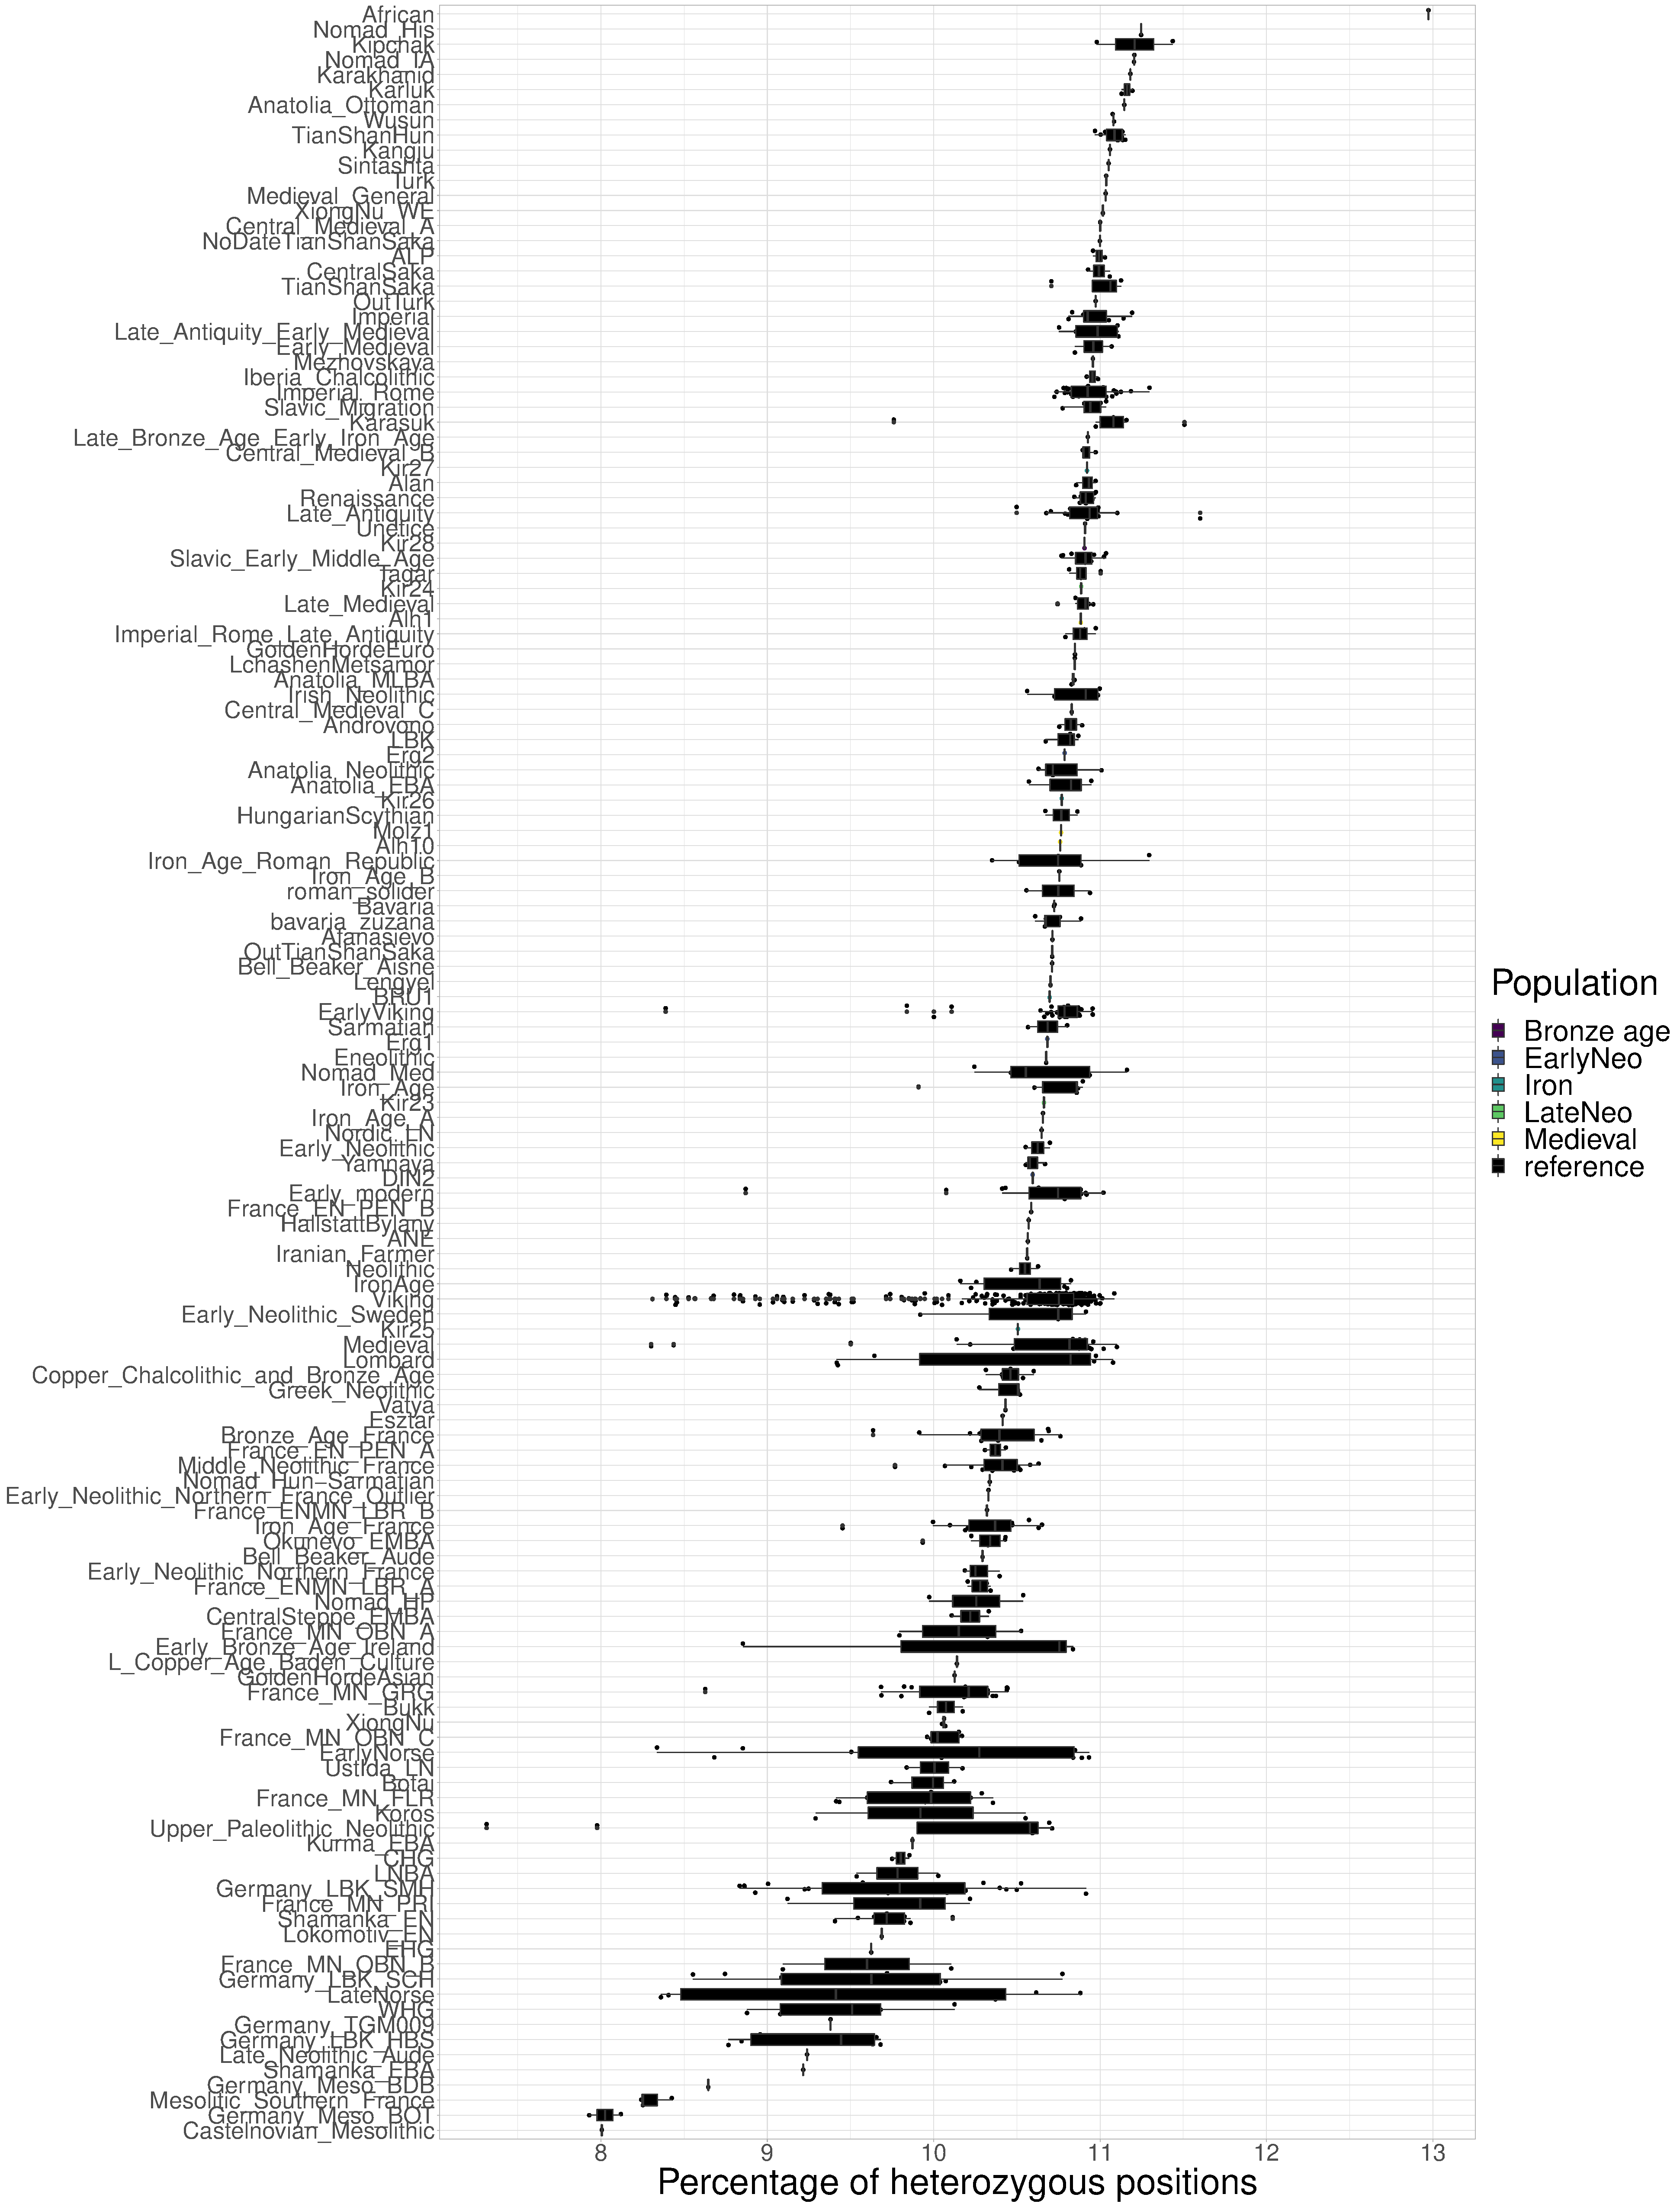
\includegraphics[width=1.0\textwidth]{../images/chapter4/het_per_pop.pdf}
    \caption{}
    \label{fig:het_per_pop}
\end{figure}

\subsection{Discussion}

I found that there was structure even within samples which were extremely spatially and temporally close. For example, Erg1 and Erg2 were found in the same layer and in the same location; yet Erg1 shows evidence of recent Hunter-Gatherer ancestry, whereas Erg2 shows no evidence of admixture. This raises the possibility that admixture between farmers and Hunter-Gatheres occured on an extremely fine geographic and tempral scale. Similarly, the two Late Neolithic samples showed differences in genetic ancestry, with one sample possibly being a recent migrant from the Eurasian Steppe, displaying ancestry typical of the Yamnaya steppe-pastoralists and the other being of primarily farmer ancestry. These results clearly demonstrate that individuals who were likely genetically and phenotypically distinct lived amongst one another during the Late Neolithic. 

I found that across the different archaeological periods, within Cherry-Tree Cave, there was a degree of continuity, but with evidence of admixture from the outside. 

Using 3 ancient genomes, I showed that the distinction between `Germanic' and `Slavic' peoples can be outlined in the context of modern samples.